\documentclass[twoside]{book}

% Packages required by doxygen
\usepackage{fixltx2e}
\usepackage{calc}
\usepackage{doxygen}
\usepackage[export]{adjustbox} % also loads graphicx
\usepackage{graphicx}
\usepackage[utf8]{inputenc}
\usepackage{makeidx}
\usepackage{multicol}
\usepackage{multirow}
\PassOptionsToPackage{warn}{textcomp}
\usepackage{textcomp}
\usepackage[nointegrals]{wasysym}
\usepackage[table]{xcolor}

% Font selection
\usepackage[T1]{fontenc}
\usepackage[scaled=.90]{helvet}
\usepackage{courier}
\usepackage{amssymb}
\usepackage{sectsty}
\renewcommand{\familydefault}{\sfdefault}
\allsectionsfont{%
  \fontseries{bc}\selectfont%
  \color{darkgray}%
}
\renewcommand{\DoxyLabelFont}{%
  \fontseries{bc}\selectfont%
  \color{darkgray}%
}
\newcommand{\+}{\discretionary{\mbox{\scriptsize$\hookleftarrow$}}{}{}}

% Page & text layout
\usepackage{geometry}
\geometry{%
  a4paper,%
  top=2.5cm,%
  bottom=2.5cm,%
  left=2.5cm,%
  right=2.5cm%
}
\tolerance=750
\hfuzz=15pt
\hbadness=750
\setlength{\emergencystretch}{15pt}
\setlength{\parindent}{0cm}
\setlength{\parskip}{3ex plus 2ex minus 2ex}
\makeatletter
\renewcommand{\paragraph}{%
  \@startsection{paragraph}{4}{0ex}{-1.0ex}{1.0ex}{%
    \normalfont\normalsize\bfseries\SS@parafont%
  }%
}
\renewcommand{\subparagraph}{%
  \@startsection{subparagraph}{5}{0ex}{-1.0ex}{1.0ex}{%
    \normalfont\normalsize\bfseries\SS@subparafont%
  }%
}
\makeatother

% Headers & footers
\usepackage{fancyhdr}
\pagestyle{fancyplain}
\fancyhead[LE]{\fancyplain{}{\bfseries\thepage}}
\fancyhead[CE]{\fancyplain{}{}}
\fancyhead[RE]{\fancyplain{}{\bfseries\leftmark}}
\fancyhead[LO]{\fancyplain{}{\bfseries\rightmark}}
\fancyhead[CO]{\fancyplain{}{}}
\fancyhead[RO]{\fancyplain{}{\bfseries\thepage}}
\fancyfoot[LE]{\fancyplain{}{}}
\fancyfoot[CE]{\fancyplain{}{}}
\fancyfoot[RE]{\fancyplain{}{\bfseries\scriptsize Generated by Doxygen }}
\fancyfoot[LO]{\fancyplain{}{\bfseries\scriptsize Generated by Doxygen }}
\fancyfoot[CO]{\fancyplain{}{}}
\fancyfoot[RO]{\fancyplain{}{}}
\renewcommand{\footrulewidth}{0.4pt}
\renewcommand{\chaptermark}[1]{%
  \markboth{#1}{}%
}
\renewcommand{\sectionmark}[1]{%
  \markright{\thesection\ #1}%
}

% Indices & bibliography
\usepackage{natbib}
\usepackage[titles]{tocloft}
\setcounter{tocdepth}{3}
\setcounter{secnumdepth}{5}
\makeindex

% Hyperlinks (required, but should be loaded last)
\usepackage{ifpdf}
\ifpdf
  \usepackage[pdftex,pagebackref=true]{hyperref}
\else
  \usepackage[ps2pdf,pagebackref=true]{hyperref}
\fi
\hypersetup{%
  colorlinks=true,%
  linkcolor=blue,%
  citecolor=blue,%
  unicode%
}

% Custom commands
\newcommand{\clearemptydoublepage}{%
  \newpage{\pagestyle{empty}\cleardoublepage}%
}

\usepackage{caption}
\captionsetup{labelsep=space,justification=centering,font={bf},singlelinecheck=off,skip=4pt,position=top}

%===== C O N T E N T S =====

\begin{document}

% Titlepage & ToC
\hypersetup{pageanchor=false,
             bookmarksnumbered=true,
             pdfencoding=unicode
            }
\pagenumbering{roman}
\begin{titlepage}
\vspace*{7cm}
\begin{center}%
{\Large C++ p\+Thread wrapper \\[1ex]\large (v1.\+2.\+0) }\\
\vspace*{1cm}
{\large Generated by Doxygen 1.8.11}\\
\end{center}
\end{titlepage}
\clearemptydoublepage
\tableofcontents
\clearemptydoublepage
\pagenumbering{arabic}
\hypersetup{pageanchor=true}

%--- Begin generated contents ---
\chapter{What it does}
\label{index}\hypertarget{index}{}I\+BM\textquotesingle{}s compiler is not implementing all the features of C++11 standard, especially it\textquotesingle{}s lacking the concurrency features that the standard brings. This will at some point be fixed and was therfore looking at a way reduce the effort to switch from a specific implementation to the C++11 standard one. This projetc is the resulting code.

This wrapper intends to bring these feature by implementing C++11 interface and using the pthread library. Of course, as it is a replacement of C++11 features, it is best to use the standard implementation if your compiler support it. This can be done rather easely by using the standard namespace {\ttfamily std} instead of this library\textquotesingle{}s specific one {\ttfamily pthread}.\+:w

To use this library\+: 
\begin{DoxyCode}
1 configure
2 make
3 make install
\end{DoxyCode}


Install moves files into your system\textquotesingle{}s default localtion of headers and libraries (often /usr/local/include and /usr/local/lib). Use this command to change target directory\+: 
\begin{DoxyCode}
1 configure --prefix=/usr/local
\end{DoxyCode}


\href{http://herbertkoelman.github.io/cpp-pthread/doc/html/}{\tt Documentation} can be generated with this command\+: 
\begin{DoxyCode}
1 make doxygen
2 ...
\end{DoxyCode}


This command creates a {\ttfamily doc} directory wich will contain the generated documentation.

\begin{quote}
{\bfseries warning} generating documentation requires that doxygen is installed. \end{quote}


\section*{How to use it}

Once compiled and installed in a location that suites you, use your compiler options to reference the headers and the libraries directory. In almoast all casses you can\+:
\begin{DoxyItemize}
\item include {\ttfamily \#include \char`\"{}pthread/phtread.\+hpp\char`\"{}} in your code.
\item comment the c++11 standard includes in your code
\item declare that you\textquotesingle{}re now using the namespace pthread ({\ttfamily using namespace pthread ;})
\end{DoxyItemize}

It should now compile use this very simple (but often good enough) implementation.

\section*{Usefull links}


\begin{DoxyItemize}
\item \href{http://pubs.opengroup.org/onlinepubs/007908799/xsh/threads.html}{\tt documentation} of the underlying P\+O\+S\+IX threading library
\item \href{https://github.com/HerbertKoelman/cpp-pthread}{\tt project\textquotesingle{}s home}
\item \href{http://herbertkoelman.github.io/cpp-pthread/doc/html/}{\tt project\textquotesingle{}s doxygen}
\item \href{http://en.cppreference.com/w/cpp/thread/thread}{\tt std\+::thread} implementation we try to mimic
\item \href{http://en.cppreference.com/w/cpp/thread/lock_guard/lock_guard}{\tt std\+::lock\+\_\+guard} implementation we try to mimic
\item \href{http://en.cppreference.com/w/cpp/thread/mutex}{\tt std\+::mutex} implementation we try to mimic
\item \href{http://en.cppreference.com/w/cpp/thread/condition_variable}{\tt std\+::condition\+\_\+variable} implementation we try to mimic
\end{DoxyItemize}

More \href{https://github.com/HerbertKoelman/cpp-pthread/wiki}{\tt here}

\section*{misc}


\begin{DoxyItemize}
\item author herbert koelman
\item github \href{https://github.com/HerbertKoelman/cpp-pthread}{\tt cpp-\/pthread} 
\end{DoxyItemize}
\chapter{Namespace Index}
\section{Namespace List}
Here is a list of all documented namespaces with brief descriptions\+:\begin{DoxyCompactList}
\item\contentsline{section}{\hyperlink{namespacepthread}{pthread} }{\pageref{namespacepthread}}{}
\item\contentsline{section}{\hyperlink{namespacepthread_1_1this__thread}{pthread\+::this\+\_\+thread} }{\pageref{namespacepthread_1_1this__thread}}{}
\end{DoxyCompactList}

\chapter{Hierarchical Index}
\section{Class Hierarchy}
This inheritance list is sorted roughly, but not completely, alphabetically\+:\begin{DoxyCompactList}
\item \contentsline{section}{pthread\+:\+:condition\+\_\+variable}{\pageref{classpthread_1_1condition__variable}}{}
\item exception\begin{DoxyCompactList}
\item \contentsline{section}{pthread\+:\+:pthread\+\_\+exception}{\pageref{classpthread_1_1pthread__exception}}{}
\begin{DoxyCompactList}
\item \contentsline{section}{pthread\+:\+:condition\+\_\+variable\+\_\+exception}{\pageref{classpthread_1_1condition__variable__exception}}{}
\item \contentsline{section}{pthread\+:\+:mutex\+\_\+exception}{\pageref{classpthread_1_1mutex__exception}}{}
\item \contentsline{section}{pthread\+:\+:thread\+\_\+exception}{\pageref{classpthread_1_1thread__exception}}{}
\item \contentsline{section}{pthread\+:\+:timeout\+\_\+exception}{\pageref{classpthread_1_1timeout__exception}}{}
\end{DoxyCompactList}
\end{DoxyCompactList}
\item \contentsline{section}{pthread\+:\+:lock\+\_\+guard$<$ Mutex\+Type $>$}{\pageref{classpthread_1_1lock__guard}}{}
\item \contentsline{section}{pthread\+:\+:mutex}{\pageref{classpthread_1_1mutex}}{}
\item \contentsline{section}{pthread\+:\+:runnable}{\pageref{classpthread_1_1runnable}}{}
\begin{DoxyCompactList}
\item \contentsline{section}{pthread\+:\+:abstract\+\_\+thread}{\pageref{classpthread_1_1abstract__thread}}{}
\end{DoxyCompactList}
\item \contentsline{section}{pthread\+:\+:thread}{\pageref{classpthread_1_1thread}}{}
\item \contentsline{section}{pthread\+:\+:thread\+\_\+group}{\pageref{classpthread_1_1thread__group}}{}
\end{DoxyCompactList}

\chapter{Class Index}
\section{Class List}
Here are the classes, structs, unions and interfaces with brief descriptions\+:\begin{DoxyCompactList}
\item\contentsline{section}{\hyperlink{classpthread_1_1abstract__thread}{pthread\+::abstract\+\_\+thread} }{\pageref{classpthread_1_1abstract__thread}}{}
\item\contentsline{section}{\hyperlink{classpthread_1_1condition__variable}{pthread\+::condition\+\_\+variable} }{\pageref{classpthread_1_1condition__variable}}{}
\item\contentsline{section}{\hyperlink{classpthread_1_1condition__variable__exception}{pthread\+::condition\+\_\+variable\+\_\+exception} }{\pageref{classpthread_1_1condition__variable__exception}}{}
\item\contentsline{section}{\hyperlink{classpthread_1_1lock__guard}{pthread\+::lock\+\_\+guard$<$ Mutex\+Type $>$} }{\pageref{classpthread_1_1lock__guard}}{}
\item\contentsline{section}{\hyperlink{classpthread_1_1mutex}{pthread\+::mutex} }{\pageref{classpthread_1_1mutex}}{}
\item\contentsline{section}{\hyperlink{classpthread_1_1mutex__exception}{pthread\+::mutex\+\_\+exception} }{\pageref{classpthread_1_1mutex__exception}}{}
\item\contentsline{section}{\hyperlink{classpthread_1_1pthread__exception}{pthread\+::pthread\+\_\+exception} }{\pageref{classpthread_1_1pthread__exception}}{}
\item\contentsline{section}{\hyperlink{classpthread_1_1runnable}{pthread\+::runnable} }{\pageref{classpthread_1_1runnable}}{}
\item\contentsline{section}{\hyperlink{classpthread_1_1thread}{pthread\+::thread} }{\pageref{classpthread_1_1thread}}{}
\item\contentsline{section}{\hyperlink{classpthread_1_1thread__exception}{pthread\+::thread\+\_\+exception} }{\pageref{classpthread_1_1thread__exception}}{}
\item\contentsline{section}{\hyperlink{classpthread_1_1thread__group}{pthread\+::thread\+\_\+group} }{\pageref{classpthread_1_1thread__group}}{}
\item\contentsline{section}{\hyperlink{classpthread_1_1timeout__exception}{pthread\+::timeout\+\_\+exception} }{\pageref{classpthread_1_1timeout__exception}}{}
\end{DoxyCompactList}

\chapter{Namespace Documentation}
\hypertarget{namespacepthread}{\section{pthread Namespace Reference}
\label{namespacepthread}\index{pthread@{pthread}}
}
\subsection*{Namespaces}
\begin{DoxyCompactItemize}
\item 
 \hyperlink{namespacepthread_1_1this__thread}{this\+\_\+thread}
\end{DoxyCompactItemize}
\subsection*{Classes}
\begin{DoxyCompactItemize}
\item 
class \hyperlink{classpthread_1_1abstract__thread}{abstract\+\_\+thread}
\item 
class \hyperlink{classpthread_1_1condition__variable}{condition\+\_\+variable}
\item 
class \hyperlink{classpthread_1_1condition__variable__exception}{condition\+\_\+variable\+\_\+exception}
\item 
class \hyperlink{classpthread_1_1lock__guard}{lock\+\_\+guard}
\item 
class \hyperlink{classpthread_1_1mutex}{mutex}
\item 
class \hyperlink{classpthread_1_1mutex__exception}{mutex\+\_\+exception}
\item 
class \hyperlink{classpthread_1_1pthread__exception}{pthread\+\_\+exception}
\item 
class \hyperlink{classpthread_1_1runnable}{runnable}
\item 
class \hyperlink{classpthread_1_1thread}{thread}
\item 
class \hyperlink{classpthread_1_1thread__exception}{thread\+\_\+exception}
\item 
class \hyperlink{classpthread_1_1thread__group}{thread\+\_\+group}
\item 
class \hyperlink{classpthread_1_1timeout__exception}{timeout\+\_\+exception}
\end{DoxyCompactItemize}
\subsection*{Enumerations}
\begin{DoxyCompactItemize}
\item 
enum \hyperlink{namespacepthread_a823f88a2bf448bd5bd5273b826830bdd}{cv\+\_\+status} \{ \hyperlink{namespacepthread_a823f88a2bf448bd5bd5273b826830bdda633b1bc5140f77a22f2c26bea4fa3398}{no\+\_\+timeout}, 
\hyperlink{namespacepthread_a823f88a2bf448bd5bd5273b826830bdda1c2d3e88a4ad820053c817753867b31a}{timedout}
 \}
\item 
enum \hyperlink{namespacepthread_ac4b6e78f3d72c946ace7a92f3bec4101}{thread\+\_\+status} \{ \hyperlink{namespacepthread_ac4b6e78f3d72c946ace7a92f3bec4101a8414cd8c988083af4eabb1311df873cf}{thread\+\_\+status\+::not\+\_\+a\+\_\+thread}, 
\hyperlink{namespacepthread_ac4b6e78f3d72c946ace7a92f3bec4101a13b3689524b86ca2caaee82399099df1}{thread\+\_\+status\+::a\+\_\+thread}
 \}
\end{DoxyCompactItemize}
\subsection*{Functions}
\begin{DoxyCompactItemize}
\item 
const char $\ast$ \hyperlink{namespacepthread_ad04d8bbcf57d64ba29047b53432a9ceb}{cpp\+\_\+pthread\+\_\+version} ()
\item 
void $\ast$ \hyperlink{namespacepthread_a4ca2138b7b0d82d63a05c708edd45a6f}{thread\+\_\+startup\+\_\+runnable} (void $\ast$)
\end{DoxyCompactItemize}


\subsection{Detailed Description}
\begin{DoxyAuthor}{Author}
herbert koelman 
\end{DoxyAuthor}
\begin{DoxyDate}{Date}
18/03/2016
\end{DoxyDate}
C++11 pthread mock implementations 

\subsection{Enumeration Type Documentation}
\hypertarget{namespacepthread_a823f88a2bf448bd5bd5273b826830bdd}{\index{pthread@{pthread}!cv\+\_\+status@{cv\+\_\+status}}
\index{cv\+\_\+status@{cv\+\_\+status}!pthread@{pthread}}
\subsubsection[{cv\+\_\+status}]{\setlength{\rightskip}{0pt plus 5cm}enum {\bf pthread\+::cv\+\_\+status}}}\label{namespacepthread_a823f88a2bf448bd5bd5273b826830bdd}
condition variable current wait status. \begin{Desc}
\item[Enumerator]\par
\begin{description}
\index{no\+\_\+timeout@{no\+\_\+timeout}!pthread@{pthread}}\index{pthread@{pthread}!no\+\_\+timeout@{no\+\_\+timeout}}\item[{\em 
\hypertarget{namespacepthread_a823f88a2bf448bd5bd5273b826830bdda633b1bc5140f77a22f2c26bea4fa3398}{no\+\_\+timeout}\label{namespacepthread_a823f88a2bf448bd5bd5273b826830bdda633b1bc5140f77a22f2c26bea4fa3398}
}]unblocked before a timeout occured \index{timedout@{timedout}!pthread@{pthread}}\index{pthread@{pthread}!timedout@{timedout}}\item[{\em 
\hypertarget{namespacepthread_a823f88a2bf448bd5bd5273b826830bdda1c2d3e88a4ad820053c817753867b31a}{timedout}\label{namespacepthread_a823f88a2bf448bd5bd5273b826830bdda1c2d3e88a4ad820053c817753867b31a}
}]condition timedout \end{description}
\end{Desc}
\hypertarget{namespacepthread_ac4b6e78f3d72c946ace7a92f3bec4101}{\index{pthread@{pthread}!thread\+\_\+status@{thread\+\_\+status}}
\index{thread\+\_\+status@{thread\+\_\+status}!pthread@{pthread}}
\subsubsection[{thread\+\_\+status}]{\setlength{\rightskip}{0pt plus 5cm}enum {\bf pthread\+::thread\+\_\+status}\hspace{0.3cm}{\ttfamily [strong]}}}\label{namespacepthread_ac4b6e78f3d72c946ace7a92f3bec4101}
current status of a thread instance \begin{Desc}
\item[Enumerator]\par
\begin{description}
\index{not\+\_\+a\+\_\+thread@{not\+\_\+a\+\_\+thread}!pthread@{pthread}}\index{pthread@{pthread}!not\+\_\+a\+\_\+thread@{not\+\_\+a\+\_\+thread}}\item[{\em 
\hypertarget{namespacepthread_ac4b6e78f3d72c946ace7a92f3bec4101a8414cd8c988083af4eabb1311df873cf}{not\+\_\+a\+\_\+thread}\label{namespacepthread_ac4b6e78f3d72c946ace7a92f3bec4101a8414cd8c988083af4eabb1311df873cf}
}]this not a thread (i.\+e. after a move operation) \index{a\+\_\+thread@{a\+\_\+thread}!pthread@{pthread}}\index{pthread@{pthread}!a\+\_\+thread@{a\+\_\+thread}}\item[{\em 
\hypertarget{namespacepthread_ac4b6e78f3d72c946ace7a92f3bec4101a13b3689524b86ca2caaee82399099df1}{a\+\_\+thread}\label{namespacepthread_ac4b6e78f3d72c946ace7a92f3bec4101a13b3689524b86ca2caaee82399099df1}
}]a valid thread \end{description}
\end{Desc}


\subsection{Function Documentation}
\hypertarget{namespacepthread_ad04d8bbcf57d64ba29047b53432a9ceb}{\index{pthread@{pthread}!cpp\+\_\+pthread\+\_\+version@{cpp\+\_\+pthread\+\_\+version}}
\index{cpp\+\_\+pthread\+\_\+version@{cpp\+\_\+pthread\+\_\+version}!pthread@{pthread}}
\subsubsection[{cpp\+\_\+pthread\+\_\+version}]{\setlength{\rightskip}{0pt plus 5cm}const char $\ast$ pthread\+::cpp\+\_\+pthread\+\_\+version (
\begin{DoxyParamCaption}
{}
\end{DoxyParamCaption}
)}}\label{namespacepthread_ad04d8bbcf57d64ba29047b53432a9ceb}
\begin{DoxyReturn}{Returns}
library version 
\end{DoxyReturn}
\hypertarget{namespacepthread_a4ca2138b7b0d82d63a05c708edd45a6f}{\index{pthread@{pthread}!thread\+\_\+startup\+\_\+runnable@{thread\+\_\+startup\+\_\+runnable}}
\index{thread\+\_\+startup\+\_\+runnable@{thread\+\_\+startup\+\_\+runnable}!pthread@{pthread}}
\subsubsection[{thread\+\_\+startup\+\_\+runnable}]{\setlength{\rightskip}{0pt plus 5cm}void $\ast$ pthread\+::thread\+\_\+startup\+\_\+runnable (
\begin{DoxyParamCaption}
\item[{void $\ast$}]{runner}
\end{DoxyParamCaption}
)}}\label{namespacepthread_a4ca2138b7b0d82d63a05c708edd45a6f}
Function used to startup a thread.

it expects a reference to a runnable instance

This function is a helper function. It has normal C linkage, and is the base for newly created Thread objects. It runs the run method on the thread object passed to it (as a void $\ast$). 
\hypertarget{namespacepthread_1_1this__thread}{}\section{pthread\+:\+:this\+\_\+thread Namespace Reference}
\label{namespacepthread_1_1this__thread}\index{pthread\+::this\+\_\+thread@{pthread\+::this\+\_\+thread}}
\subsection*{Functions}
\begin{DoxyCompactItemize}
\item 
void \hyperlink{group__threads_ga01ae1b738d3d2dbbfe966b4aad07a0a9}{sleep\+\_\+for} (const int millis)
\item 
pthread\+\_\+t \hyperlink{group__threads_ga57275c7fa3dd5591c7f19ccf451f1fb6}{get\+\_\+id} ()
\end{DoxyCompactItemize}


\subsection{Detailed Description}
helper functions \begin{DoxyAuthor}{Author}
herbert koelman (\href{mailto:herbert.koelman@me.com}{\tt herbert.\+koelman@me.\+com}) 
\end{DoxyAuthor}

\chapter{Class Documentation}
\hypertarget{classpthread_1_1abstract__thread}{}\section{pthread\+:\+:abstract\+\_\+thread Class Reference}
\label{classpthread_1_1abstract__thread}\index{pthread\+::abstract\+\_\+thread@{pthread\+::abstract\+\_\+thread}}


{\ttfamily \#include $<$thread.\+hpp$>$}

Inheritance diagram for pthread\+:\+:abstract\+\_\+thread\+:\begin{figure}[H]
\begin{center}
\leavevmode
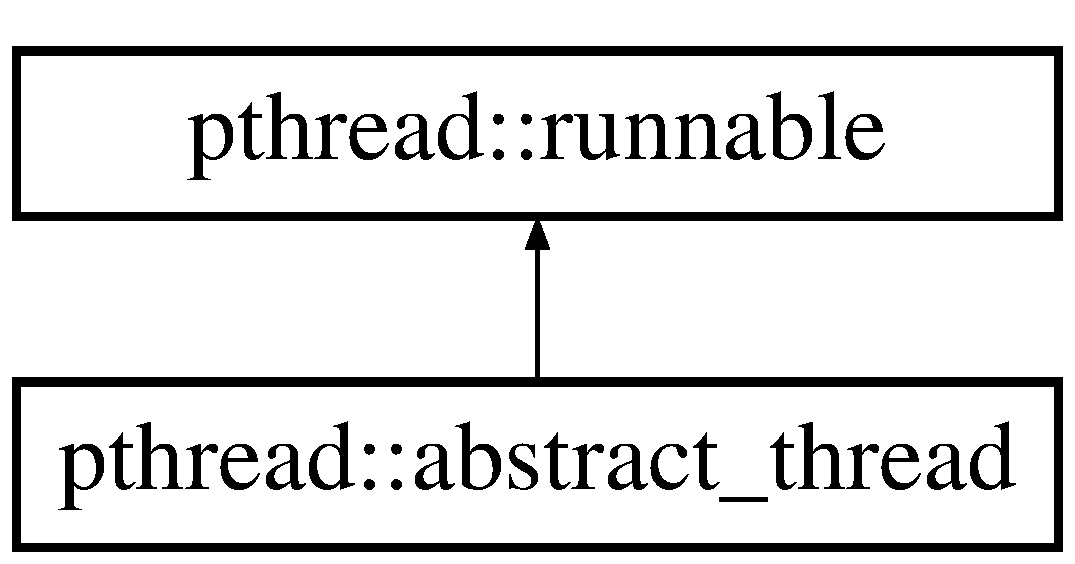
\includegraphics[height=2.000000cm]{classpthread_1_1abstract__thread}
\end{center}
\end{figure}
\subsection*{Public Member Functions}
\begin{DoxyCompactItemize}
\item 
void \hyperlink{classpthread_1_1abstract__thread_ab121718028f3ca68d45db84d10ff2a3a}{start} ()
\item 
int \hyperlink{classpthread_1_1abstract__thread_aedac81bb9eb76ba92c49c48d797ea25b}{join} ()
\end{DoxyCompactItemize}


\subsection{Detailed Description}
base class of a thread.

utility class, that wraps a thread. 
\begin{DoxyPre}{\ttfamily 
class worker: public \hyperlink{classpthread_1_1abstract__thread}{pthread::abstract\_thread} \{
public:}\end{DoxyPre}



\begin{DoxyPre}{\ttfamily   worker(const std::string m = "anonymous worker", int sleep = 2*1000): msg(m), \_sleep(sleep)\{
  \};}\end{DoxyPre}



\begin{DoxyPre}{\ttfamily   ~worker()\{
  \};}\end{DoxyPre}



\begin{DoxyPre}{\ttfamily   void \hyperlink{classpthread_1_1runnable_ad5cfd01857f1d51c42d6a16d09efe930}{run()} noexcept override \{
    \{ // critical section scope
      pthread::lock\_guard<pthread::mutex> lck(mtx);}\end{DoxyPre}



\begin{DoxyPre}{\ttfamily       bool stop\_waiting = true; // if lambda syntax is not availbale then use this kind of implementation
      auto delay = \_sleep; // use sleep seconds to calculate point in time timeout
      while ( ! (stop\_waiting = (counter >= 10000)) \&\& (condition.wait\_for(mtx, delay) == pthread::cv\_status::no\_timeout))\{
        delay = -1 ; // if timeout millis is negatif, then we keep last timeout calculation.
      \}}\end{DoxyPre}



\begin{DoxyPre}{\ttfamily       if ( counter >= 10000 ) \{
        message("worker class, counter >= 10000");
      \} else \{
        message("worker class, counter < 10000");
      \}
    \} // end of critical section}\end{DoxyPre}



\begin{DoxyPre}{\ttfamily     pthread::this\_thread::sleep(200);
  \};}\end{DoxyPre}



\begin{DoxyPre}{\ttfamily private:
  std::string    msg ;
  int            \_sleep;
\};}\end{DoxyPre}



\begin{DoxyPre}{\ttfamily int main(int argc, const char * argv[]) \{}\end{DoxyPre}



\begin{DoxyPre}{\ttfamily   \hyperlink{classpthread_1_1thread__group}{pthread::thread\_group} threads(true); // indicate that we want to join referenced threads when deallocating this instance.
  for (auto x = 10 ; x > 0 ; x--)\{
    threads.add( new worker("herbert"));
  \}}\end{DoxyPre}



\begin{DoxyPre}{\ttfamily   threads.start(); // start running all threads}\end{DoxyPre}



\begin{DoxyPre}{\ttfamily   for ( auto x = 20000 ; x > 0 ; x--)\{
    pthread::lock\_guard<pthread::mutex> lck(mtx);
    counter++ ;
  \}}\end{DoxyPre}



\begin{DoxyPre}{\ttfamily   condition.notify\_all();
\}}\end{DoxyPre}



\begin{DoxyPre}{\ttfamily }\end{DoxyPre}
 

\subsection{Member Function Documentation}
\index{pthread\+::abstract\+\_\+thread@{pthread\+::abstract\+\_\+thread}!join@{join}}
\index{join@{join}!pthread\+::abstract\+\_\+thread@{pthread\+::abstract\+\_\+thread}}
\subsubsection[{\texorpdfstring{join()}{join()}}]{\setlength{\rightskip}{0pt plus 5cm}int pthread\+::abstract\+\_\+thread\+::join (
\begin{DoxyParamCaption}
{}
\end{DoxyParamCaption}
)\hspace{0.3cm}{\ttfamily [inline]}}\hypertarget{classpthread_1_1abstract__thread_aedac81bb9eb76ba92c49c48d797ea25b}{}\label{classpthread_1_1abstract__thread_aedac81bb9eb76ba92c49c48d797ea25b}
joins this thread.

an exception is thrown if deadlock condition are detected. \index{pthread\+::abstract\+\_\+thread@{pthread\+::abstract\+\_\+thread}!start@{start}}
\index{start@{start}!pthread\+::abstract\+\_\+thread@{pthread\+::abstract\+\_\+thread}}
\subsubsection[{\texorpdfstring{start()}{start()}}]{\setlength{\rightskip}{0pt plus 5cm}void pthread\+::abstract\+\_\+thread\+::start (
\begin{DoxyParamCaption}
{}
\end{DoxyParamCaption}
)}\hypertarget{classpthread_1_1abstract__thread_ab121718028f3ca68d45db84d10ff2a3a}{}\label{classpthread_1_1abstract__thread_ab121718028f3ca68d45db84d10ff2a3a}
start running the {\ttfamily \hyperlink{classpthread_1_1runnable_ad5cfd01857f1d51c42d6a16d09efe930}{run()}} method in a new thread. 

The documentation for this class was generated from the following files\+:\begin{DoxyCompactItemize}
\item 
include/pthread/thread.\+hpp\item 
src/thread.\+cpp\end{DoxyCompactItemize}

\hypertarget{classpthread_1_1condition__variable}{}\section{pthread\+:\+:condition\+\_\+variable Class Reference}
\label{classpthread_1_1condition__variable}\index{pthread\+::condition\+\_\+variable@{pthread\+::condition\+\_\+variable}}


{\ttfamily \#include $<$condition\+\_\+variable.\+hpp$>$}

\subsection*{Public Member Functions}
\begin{DoxyCompactItemize}
\item 
void \hyperlink{classpthread_1_1condition__variable_a34247dacb9da1856f3a65bc868b6abb8}{wait} (\hyperlink{classpthread_1_1mutex}{mutex} \&mtx)
\item 
void \hyperlink{classpthread_1_1condition__variable_a9bb3e49f17ec1470c305d8b21daadf2a}{wait} (\hyperlink{classpthread_1_1lock__guard}{lock\+\_\+guard}$<$ \hyperlink{classpthread_1_1mutex}{pthread\+::mutex} $>$ lck)
\item 
{\footnotesize template$<$class Lambda $>$ }\\bool \hyperlink{classpthread_1_1condition__variable_a251a506415355171be3052b68bc8d2ec}{wait} (\hyperlink{classpthread_1_1mutex}{mutex} \&mtx, Lambda lambda)
\item 
{\footnotesize template$<$class Lambda $>$ }\\bool \hyperlink{classpthread_1_1condition__variable_a7b6c075d1588178301547bc60c59ceba}{wait} (\hyperlink{classpthread_1_1lock__guard}{lock\+\_\+guard}$<$ \hyperlink{classpthread_1_1mutex}{pthread\+::mutex} $>$ \&lck, Lambda lambda)
\item 
\hyperlink{namespacepthread_a823f88a2bf448bd5bd5273b826830bdd}{cv\+\_\+status} \hyperlink{classpthread_1_1condition__variable_a804a305eefb4da8abecd1e6326b82785}{wait\+\_\+for} (\hyperlink{classpthread_1_1mutex}{mutex} \&mtx, int millis)
\item 
\hyperlink{namespacepthread_a823f88a2bf448bd5bd5273b826830bdd}{cv\+\_\+status} \hyperlink{classpthread_1_1condition__variable_a1dfcedf00e9822587c7b20da9c060fd9}{wait\+\_\+for} (\hyperlink{classpthread_1_1lock__guard}{lock\+\_\+guard}$<$ \hyperlink{classpthread_1_1mutex}{pthread\+::mutex} $>$ \&lck, int millis)
\item 
{\footnotesize template$<$class Lambda $>$ }\\bool \hyperlink{classpthread_1_1condition__variable_a82fb3ff516ffef37c68f58e277fad855}{wait\+\_\+for} (\hyperlink{classpthread_1_1mutex}{mutex} \&mtx, int millis, Lambda lambda)
\item 
{\footnotesize template$<$class Lambda $>$ }\\bool \hyperlink{classpthread_1_1condition__variable_a5ee32edbf76592ec443e2544ecba811a}{wait\+\_\+for} (\hyperlink{classpthread_1_1lock__guard}{lock\+\_\+guard}$<$ \hyperlink{classpthread_1_1mutex}{pthread\+::mutex} $>$ \&lck, int millis, Lambda lambda)
\item 
void \hyperlink{classpthread_1_1condition__variable_ae374b1e852f36fc5eac93ad90d9fc85a}{notify\+\_\+one} () noexcept
\item 
void \hyperlink{classpthread_1_1condition__variable_ae40f0c9043ed693317bb9a07861efc65}{notify\+\_\+all} () noexcept
\end{DoxyCompactItemize}


\subsection{Detailed Description}
pthread condition variable

The \hyperlink{classpthread_1_1condition__variable}{condition\+\_\+variable} class is a synchronization primitive that can be used to block a thread, or multiple threads at the same time, until another thread both modifies a shared variable (the condition), and notifies the \hyperlink{classpthread_1_1condition__variable}{condition\+\_\+variable}.

The thread that intends to modify the variable has to
\begin{DoxyItemize}
\item acquire a std\+::mutex (typically via std\+::lock\+\_\+guard)
\item perform the modification while the lock is held
\item execute notify\+\_\+one or notify\+\_\+all on the std\+::condition\+\_\+variable (the lock does not need to be held for notification)
\end{DoxyItemize}

Even if the shared variable is atomic, it must be modified under the mutex in order to correctly publish the modification to the waiting thread.

Upon successful return, the mutex shall have been locked and shall be owned by the calling thread.

\begin{DoxyAuthor}{Author}
herbert koelman 
\end{DoxyAuthor}


\subsection{Member Function Documentation}
\index{pthread\+::condition\+\_\+variable@{pthread\+::condition\+\_\+variable}!notify\+\_\+all@{notify\+\_\+all}}
\index{notify\+\_\+all@{notify\+\_\+all}!pthread\+::condition\+\_\+variable@{pthread\+::condition\+\_\+variable}}
\subsubsection[{\texorpdfstring{notify\+\_\+all() noexcept}{notify_all() noexcept}}]{\setlength{\rightskip}{0pt plus 5cm}void pthread\+::condition\+\_\+variable\+::notify\+\_\+all (
\begin{DoxyParamCaption}
{}
\end{DoxyParamCaption}
)\hspace{0.3cm}{\ttfamily [noexcept]}}\hypertarget{classpthread_1_1condition__variable_ae40f0c9043ed693317bb9a07861efc65}{}\label{classpthread_1_1condition__variable_ae40f0c9043ed693317bb9a07861efc65}
signal all waiting threads The pthread\+\_\+cond\+\_\+broadcast() call unblocks all threads currently blocked on the specified condition variable cond. \index{pthread\+::condition\+\_\+variable@{pthread\+::condition\+\_\+variable}!notify\+\_\+one@{notify\+\_\+one}}
\index{notify\+\_\+one@{notify\+\_\+one}!pthread\+::condition\+\_\+variable@{pthread\+::condition\+\_\+variable}}
\subsubsection[{\texorpdfstring{notify\+\_\+one() noexcept}{notify_one() noexcept}}]{\setlength{\rightskip}{0pt plus 5cm}void pthread\+::condition\+\_\+variable\+::notify\+\_\+one (
\begin{DoxyParamCaption}
{}
\end{DoxyParamCaption}
)\hspace{0.3cm}{\ttfamily [noexcept]}}\hypertarget{classpthread_1_1condition__variable_ae374b1e852f36fc5eac93ad90d9fc85a}{}\label{classpthread_1_1condition__variable_ae374b1e852f36fc5eac93ad90d9fc85a}
signal one waiting thread.

The pthread\+\_\+cond\+\_\+signal() call unblocks at least one of the threads that are blocked on the specified condition variable cond (if any threads are blocked on cond). \index{pthread\+::condition\+\_\+variable@{pthread\+::condition\+\_\+variable}!wait@{wait}}
\index{wait@{wait}!pthread\+::condition\+\_\+variable@{pthread\+::condition\+\_\+variable}}
\subsubsection[{\texorpdfstring{wait(mutex \&mtx)}{wait(mutex &mtx)}}]{\setlength{\rightskip}{0pt plus 5cm}void pthread\+::condition\+\_\+variable\+::wait (
\begin{DoxyParamCaption}
\item[{{\bf mutex} \&}]{mtx}
\end{DoxyParamCaption}
)}\hypertarget{classpthread_1_1condition__variable_a34247dacb9da1856f3a65bc868b6abb8}{}\label{classpthread_1_1condition__variable_a34247dacb9da1856f3a65bc868b6abb8}
wait for condition to be signaled

This method atomically release mutex and cause the calling thread to block; atomically here means \char`\"{}atomically with respect to
access by another thread to the mutex and then the condition variable\char`\"{}. Call notify\+\_\+one or notify\+\_\+all to signal the condition.

Upon successful return, the mutex has been locked and is owned by the calling thread.


\begin{DoxyParams}{Parameters}
{\em mtx} & ralated mutex, which must be locked by the current thread. \\
\hline
\end{DoxyParams}
\index{pthread\+::condition\+\_\+variable@{pthread\+::condition\+\_\+variable}!wait@{wait}}
\index{wait@{wait}!pthread\+::condition\+\_\+variable@{pthread\+::condition\+\_\+variable}}
\subsubsection[{\texorpdfstring{wait(lock\+\_\+guard$<$ pthread\+::mutex $>$ lck)}{wait(lock_guard< pthread::mutex > lck)}}]{\setlength{\rightskip}{0pt plus 5cm}void pthread\+::condition\+\_\+variable\+::wait (
\begin{DoxyParamCaption}
\item[{{\bf lock\+\_\+guard}$<$ {\bf pthread\+::mutex} $>$}]{lck}
\end{DoxyParamCaption}
)}\hypertarget{classpthread_1_1condition__variable_a9bb3e49f17ec1470c305d8b21daadf2a}{}\label{classpthread_1_1condition__variable_a9bb3e49f17ec1470c305d8b21daadf2a}
\begin{DoxySeeAlso}{See also}
\hyperlink{classpthread_1_1condition__variable_a34247dacb9da1856f3a65bc868b6abb8}{wait} 
\end{DoxySeeAlso}
\index{pthread\+::condition\+\_\+variable@{pthread\+::condition\+\_\+variable}!wait@{wait}}
\index{wait@{wait}!pthread\+::condition\+\_\+variable@{pthread\+::condition\+\_\+variable}}
\subsubsection[{\texorpdfstring{wait(mutex \&mtx, Lambda lambda)}{wait(mutex &mtx, Lambda lambda)}}]{\setlength{\rightskip}{0pt plus 5cm}template$<$class Lambda $>$ bool pthread\+::condition\+\_\+variable\+::wait (
\begin{DoxyParamCaption}
\item[{{\bf mutex} \&}]{mtx, }
\item[{Lambda}]{lambda}
\end{DoxyParamCaption}
)}\hypertarget{classpthread_1_1condition__variable_a251a506415355171be3052b68bc8d2ec}{}\label{classpthread_1_1condition__variable_a251a506415355171be3052b68bc8d2ec}
wait for condition to be signaled

This method atomically release mutex and cause the calling thread to block; atomically here means \char`\"{}atomically with respect to
access by another thread to the mutex and then the condition variable\char`\"{}. Call notify\+\_\+one or notify\+\_\+all to signal the condition.

Upon successful return, the mutex has been locked and is owned by the calling thread.

The lambda (closure) is run to check if the condition was met. Lambda should false if the waiting should be continued. The signature of the predicate function should be equivalent to the following\+: bool pred();


\begin{DoxyParams}{Parameters}
{\em mtx} & ralated mutex, which must be locked by the current thread. \\
\hline
{\em lambda} & run to check if condition was met. \\
\hline
\end{DoxyParams}
\begin{DoxyReturn}{Returns}
true if lmabda returned true. 
\end{DoxyReturn}
\index{pthread\+::condition\+\_\+variable@{pthread\+::condition\+\_\+variable}!wait@{wait}}
\index{wait@{wait}!pthread\+::condition\+\_\+variable@{pthread\+::condition\+\_\+variable}}
\subsubsection[{\texorpdfstring{wait(lock\+\_\+guard$<$ pthread\+::mutex $>$ \&lck, Lambda lambda)}{wait(lock_guard< pthread::mutex > &lck, Lambda lambda)}}]{\setlength{\rightskip}{0pt plus 5cm}template$<$class Lambda $>$ bool pthread\+::condition\+\_\+variable\+::wait (
\begin{DoxyParamCaption}
\item[{{\bf lock\+\_\+guard}$<$ {\bf pthread\+::mutex} $>$ \&}]{lck, }
\item[{Lambda}]{lambda}
\end{DoxyParamCaption}
)}\hypertarget{classpthread_1_1condition__variable_a7b6c075d1588178301547bc60c59ceba}{}\label{classpthread_1_1condition__variable_a7b6c075d1588178301547bc60c59ceba}
wait for condition to be signaled

This method atomically release mutex and cause the calling thread to block; atomically here means \char`\"{}atomically with respect to
access by another thread to the mutex and then the condition variable\char`\"{}. Call notify\+\_\+one or notify\+\_\+all to signal the condition.

Upon successful return, the mutex has been locked and is owned by the calling thread.

The lambda (closure) is run to check if the condition was met. Lambda should false if the waiting should be continued. The signature of the predicate function should be equivalent to the following\+: bool pred();


\begin{DoxyParams}{Parameters}
{\em lck} & ralated mutex \hyperlink{classpthread_1_1lock__guard}{lock\+\_\+guard}, which must be locked by the current thread. \\
\hline
{\em lambda} & run to check if condition was met. \\
\hline
\end{DoxyParams}
\begin{DoxyReturn}{Returns}
true if lmabda returned true. 
\end{DoxyReturn}
\index{pthread\+::condition\+\_\+variable@{pthread\+::condition\+\_\+variable}!wait\+\_\+for@{wait\+\_\+for}}
\index{wait\+\_\+for@{wait\+\_\+for}!pthread\+::condition\+\_\+variable@{pthread\+::condition\+\_\+variable}}
\subsubsection[{\texorpdfstring{wait\+\_\+for(mutex \&mtx, int millis)}{wait_for(mutex &mtx, int millis)}}]{\setlength{\rightskip}{0pt plus 5cm}{\bf cv\+\_\+status} pthread\+::condition\+\_\+variable\+::wait\+\_\+for (
\begin{DoxyParamCaption}
\item[{{\bf mutex} \&}]{mtx, }
\item[{int}]{millis}
\end{DoxyParamCaption}
)}\hypertarget{classpthread_1_1condition__variable_a804a305eefb4da8abecd1e6326b82785}{}\label{classpthread_1_1condition__variable_a804a305eefb4da8abecd1e6326b82785}
wait for condition to be signaled within given time frame

This method atomically release mutex and cause the calling thread to block; atomically here means \char`\"{}atomically with respect to
access by another thread to the mutex and then the condition variable\char`\"{}. Call notify\+\_\+one or notify\+\_\+all to signal the condition.

Upon successful return, the mutex has been locked and is owned by the calling thread.


\begin{DoxyParams}{Parameters}
{\em mtx} & ralated mutex, which must be locked by the current thread. \\
\hline
{\em millis} & milliseconds to wait for this instance to signaled. \\
\hline
\end{DoxyParams}
\begin{DoxyReturn}{Returns}
cv\+\_\+status (either timeout or no\+\_\+timeout) 
\end{DoxyReturn}
\index{pthread\+::condition\+\_\+variable@{pthread\+::condition\+\_\+variable}!wait\+\_\+for@{wait\+\_\+for}}
\index{wait\+\_\+for@{wait\+\_\+for}!pthread\+::condition\+\_\+variable@{pthread\+::condition\+\_\+variable}}
\subsubsection[{\texorpdfstring{wait\+\_\+for(lock\+\_\+guard$<$ pthread\+::mutex $>$ \&lck, int millis)}{wait_for(lock_guard< pthread::mutex > &lck, int millis)}}]{\setlength{\rightskip}{0pt plus 5cm}{\bf cv\+\_\+status} pthread\+::condition\+\_\+variable\+::wait\+\_\+for (
\begin{DoxyParamCaption}
\item[{{\bf lock\+\_\+guard}$<$ {\bf pthread\+::mutex} $>$ \&}]{lck, }
\item[{int}]{millis}
\end{DoxyParamCaption}
)}\hypertarget{classpthread_1_1condition__variable_a1dfcedf00e9822587c7b20da9c060fd9}{}\label{classpthread_1_1condition__variable_a1dfcedf00e9822587c7b20da9c060fd9}
\begin{DoxySeeAlso}{See also}
\hyperlink{classpthread_1_1condition__variable_a804a305eefb4da8abecd1e6326b82785}{wait\+\_\+for} (\hyperlink{classpthread_1_1mutex}{mutex} \&, int) 
\end{DoxySeeAlso}
\index{pthread\+::condition\+\_\+variable@{pthread\+::condition\+\_\+variable}!wait\+\_\+for@{wait\+\_\+for}}
\index{wait\+\_\+for@{wait\+\_\+for}!pthread\+::condition\+\_\+variable@{pthread\+::condition\+\_\+variable}}
\subsubsection[{\texorpdfstring{wait\+\_\+for(mutex \&mtx, int millis, Lambda lambda)}{wait_for(mutex &mtx, int millis, Lambda lambda)}}]{\setlength{\rightskip}{0pt plus 5cm}template$<$class Lambda $>$ bool pthread\+::condition\+\_\+variable\+::wait\+\_\+for (
\begin{DoxyParamCaption}
\item[{{\bf mutex} \&}]{mtx, }
\item[{int}]{millis, }
\item[{Lambda}]{lambda}
\end{DoxyParamCaption}
)}\hypertarget{classpthread_1_1condition__variable_a82fb3ff516ffef37c68f58e277fad855}{}\label{classpthread_1_1condition__variable_a82fb3ff516ffef37c68f58e277fad855}
wait for condition to be signaled within a given time frame

This method atomically release mutex and cause the calling thread to block; atomically here means \char`\"{}atomically with respect to
access by another thread to the mutex and then the condition variable\char`\"{}. Call notify\+\_\+one or notify\+\_\+all to signal the condition.

Upon successful return, the mutex has been locked and is owned by the calling thread.

The lambda (closure) is run to check if the condition was met. Lambda should false if the waiting should be continued. The signature of the predicate function should be equivalent to the following\+: bool lambda();


\begin{DoxyParams}{Parameters}
{\em mtx} & ralated mutex, which must be locked by the current thread. \\
\hline
{\em millis} & milli seconds to wait for condition to be signaled. \\
\hline
{\em lambda} & run to check if condition was met. \\
\hline
\end{DoxyParams}
\begin{DoxyReturn}{Returns}
true if lmabda returned true. 
\end{DoxyReturn}
\index{pthread\+::condition\+\_\+variable@{pthread\+::condition\+\_\+variable}!wait\+\_\+for@{wait\+\_\+for}}
\index{wait\+\_\+for@{wait\+\_\+for}!pthread\+::condition\+\_\+variable@{pthread\+::condition\+\_\+variable}}
\subsubsection[{\texorpdfstring{wait\+\_\+for(lock\+\_\+guard$<$ pthread\+::mutex $>$ \&lck, int millis, Lambda lambda)}{wait_for(lock_guard< pthread::mutex > &lck, int millis, Lambda lambda)}}]{\setlength{\rightskip}{0pt plus 5cm}template$<$class Lambda $>$ bool pthread\+::condition\+\_\+variable\+::wait\+\_\+for (
\begin{DoxyParamCaption}
\item[{{\bf lock\+\_\+guard}$<$ {\bf pthread\+::mutex} $>$ \&}]{lck, }
\item[{int}]{millis, }
\item[{Lambda}]{lambda}
\end{DoxyParamCaption}
)}\hypertarget{classpthread_1_1condition__variable_a5ee32edbf76592ec443e2544ecba811a}{}\label{classpthread_1_1condition__variable_a5ee32edbf76592ec443e2544ecba811a}
wait for condition to be signaled within a given time frame

This method atomically release mutex and cause the calling thread to block; atomically here means \char`\"{}atomically with respect to
access by another thread to the mutex and then the condition variable\char`\"{}. Call notify\+\_\+one or notify\+\_\+all to signal the condition.

Upon successful return, the mutex has been locked and is owned by the calling thread.

The lambda (closure) is run to check if the condition was met. Lambda should false if the waiting should be continued. The signature of the predicate function should be equivalent to the following\+: bool lambda();


\begin{DoxyParams}{Parameters}
{\em lck} & ralated mutex \hyperlink{classpthread_1_1lock__guard}{lock\+\_\+guard}, which must be locked by the current thread. \\
\hline
{\em millis} & milli seconds to wait for condition to be signaled. \\
\hline
{\em lambda} & run to check if condition was met. \\
\hline
\end{DoxyParams}
\begin{DoxyReturn}{Returns}
true if lmabda returned true. 
\end{DoxyReturn}


The documentation for this class was generated from the following files\+:\begin{DoxyCompactItemize}
\item 
include/pthread/condition\+\_\+variable.\+hpp\item 
src/condition\+\_\+variable.\+cpp\end{DoxyCompactItemize}

\hypertarget{classpthread_1_1condition__variable__exception}{\section{pthread\+:\+:condition\+\_\+variable\+\_\+exception Class Reference}
\label{classpthread_1_1condition__variable__exception}\index{pthread\+::condition\+\_\+variable\+\_\+exception@{pthread\+::condition\+\_\+variable\+\_\+exception}}
}


{\ttfamily \#include $<$exceptions.\+hpp$>$}

Inheritance diagram for pthread\+:\+:condition\+\_\+variable\+\_\+exception\+:\begin{figure}[H]
\begin{center}
\leavevmode
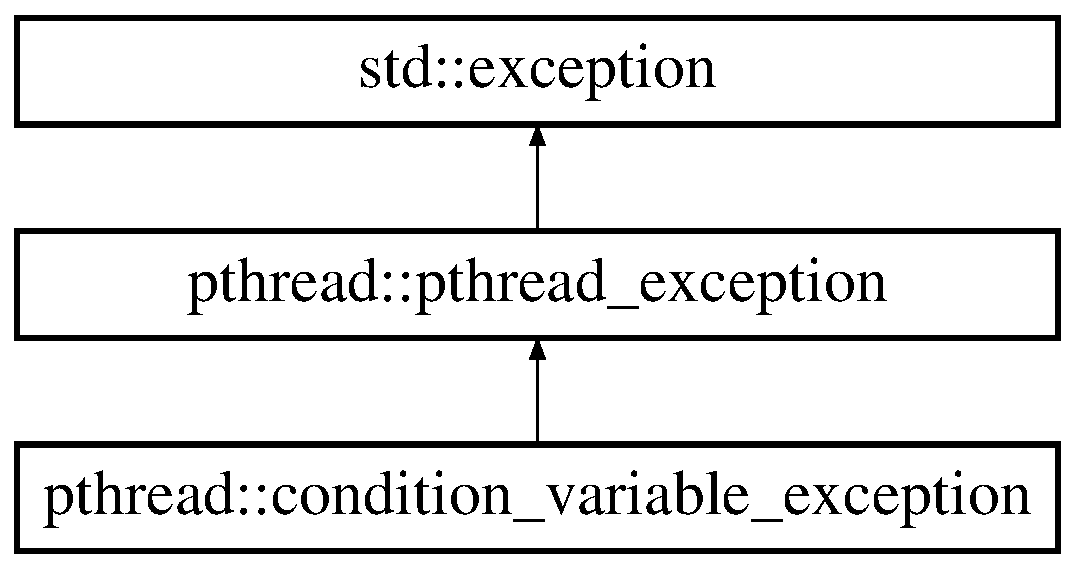
\includegraphics[height=3.000000cm]{classpthread_1_1condition__variable__exception}
\end{center}
\end{figure}
\subsection*{Public Member Functions}
\begin{DoxyCompactItemize}
\item 
\hyperlink{classpthread_1_1condition__variable__exception_a5405694c69de500c7c6fdaba3e3af8a5}{condition\+\_\+variable\+\_\+exception} (const std\+::string \&message, const int \hyperlink{classpthread_1_1pthread__exception_a4a869173054faca1945ac1a7729082d6}{pthread\+\_\+errno}=-\/1)
\end{DoxyCompactItemize}


\subsection{Detailed Description}
Condition variable exception 

Definition at line 108 of file exceptions.\+hpp.



\subsection{Constructor \& Destructor Documentation}
\hypertarget{classpthread_1_1condition__variable__exception_a5405694c69de500c7c6fdaba3e3af8a5}{\index{pthread\+::condition\+\_\+variable\+\_\+exception@{pthread\+::condition\+\_\+variable\+\_\+exception}!condition\+\_\+variable\+\_\+exception@{condition\+\_\+variable\+\_\+exception}}
\index{condition\+\_\+variable\+\_\+exception@{condition\+\_\+variable\+\_\+exception}!pthread\+::condition\+\_\+variable\+\_\+exception@{pthread\+::condition\+\_\+variable\+\_\+exception}}
\subsubsection[{condition\+\_\+variable\+\_\+exception}]{\setlength{\rightskip}{0pt plus 5cm}pthread\+::condition\+\_\+variable\+\_\+exception\+::condition\+\_\+variable\+\_\+exception (
\begin{DoxyParamCaption}
\item[{const std\+::string \&}]{message, }
\item[{const int}]{pthread\+\_\+errno = {\ttfamily -\/1}}
\end{DoxyParamCaption}
)}}\label{classpthread_1_1condition__variable__exception_a5405694c69de500c7c6fdaba3e3af8a5}
thrown when mutex actions fail


\begin{DoxyParams}{Parameters}
{\em message} & short description \\
\hline
{\em pthread\+\_\+errno} & error returned by the pthread function \\
\hline
\end{DoxyParams}


Definition at line 57 of file exceptions.\+cpp.



The documentation for this class was generated from the following files\+:\begin{DoxyCompactItemize}
\item 
include/pthread/exceptions.\+hpp\item 
src/exceptions.\+cpp\end{DoxyCompactItemize}

\hypertarget{classpthread_1_1lock__guard}{}\section{pthread\+:\+:lock\+\_\+guard$<$ Mutex\+Type $>$ Class Template Reference}
\label{classpthread_1_1lock__guard}\index{pthread\+::lock\+\_\+guard$<$ Mutex\+Type $>$@{pthread\+::lock\+\_\+guard$<$ Mutex\+Type $>$}}


{\ttfamily \#include $<$lock\+\_\+guard.\+hpp$>$}

\subsection*{Public Member Functions}
\begin{DoxyCompactItemize}
\item 
\hyperlink{classpthread_1_1lock__guard_a720070a45ed97c9234b980bd33328a4e}{lock\+\_\+guard} (\hyperlink{classpthread_1_1mutex}{mutex} \&m)
\item 
\hyperlink{classpthread_1_1lock__guard_a958884251adfb8d5f9bd7d643cc3949f}{$\sim$lock\+\_\+guard} ()
\item 
void {\bfseries operator=} (\hyperlink{classpthread_1_1lock__guard}{lock\+\_\+guard} \&)=delete\hypertarget{classpthread_1_1lock__guard_a1f9ab705f7ffe9eb8739ff3cf34cf7f2}{}\label{classpthread_1_1lock__guard_a1f9ab705f7ffe9eb8739ff3cf34cf7f2}

\item 
Mutex\+Type $\ast$ \hyperlink{classpthread_1_1lock__guard_a03f11b486e905ea9bca764686cd86fae}{mutex} () const 
\end{DoxyCompactItemize}


\subsection{Detailed Description}
\subsubsection*{template$<$class Mutex\+Type$>$\\*
class pthread\+::lock\+\_\+guard$<$ Mutex\+Type $>$}

This class was designed to encapsulate a mutex and automatically control the lock attribute.

The \hyperlink{classpthread_1_1lock__guard}{lock\+\_\+guard} lock the associated mutex once we instanciate the class and the lock is automatically unlocked once the object is destroyed. This allow us to correlate the lock with the scope of the object.

\begin{DoxyAuthor}{Author}
herbert koelman 
\end{DoxyAuthor}


\subsection{Constructor \& Destructor Documentation}
\index{pthread\+::lock\+\_\+guard@{pthread\+::lock\+\_\+guard}!lock\+\_\+guard@{lock\+\_\+guard}}
\index{lock\+\_\+guard@{lock\+\_\+guard}!pthread\+::lock\+\_\+guard@{pthread\+::lock\+\_\+guard}}
\subsubsection[{\texorpdfstring{lock\+\_\+guard(mutex \&m)}{lock_guard(mutex &m)}}]{\setlength{\rightskip}{0pt plus 5cm}template$<$class Mutex\+Type$>$ {\bf pthread\+::lock\+\_\+guard}$<$ Mutex\+Type $>$\+::{\bf lock\+\_\+guard} (
\begin{DoxyParamCaption}
\item[{{\bf mutex} \&}]{m}
\end{DoxyParamCaption}
)\hspace{0.3cm}{\ttfamily [inline]}, {\ttfamily [explicit]}}\hypertarget{classpthread_1_1lock__guard_a720070a45ed97c9234b980bd33328a4e}{}\label{classpthread_1_1lock__guard_a720070a45ed97c9234b980bd33328a4e}
The constructor is forced to only accept a mutex object or any object of a subclass.

The mutex is locked up completion.


\begin{DoxyParams}{Parameters}
{\em m} & reference to a valid \hyperlink{classpthread_1_1mutex}{pthread\+::mutex} \\
\hline
\end{DoxyParams}
\index{pthread\+::lock\+\_\+guard@{pthread\+::lock\+\_\+guard}!````~lock\+\_\+guard@{$\sim$lock\+\_\+guard}}
\index{````~lock\+\_\+guard@{$\sim$lock\+\_\+guard}!pthread\+::lock\+\_\+guard@{pthread\+::lock\+\_\+guard}}
\subsubsection[{\texorpdfstring{$\sim$lock\+\_\+guard()}{~lock_guard()}}]{\setlength{\rightskip}{0pt plus 5cm}template$<$class Mutex\+Type$>$ {\bf pthread\+::lock\+\_\+guard}$<$ Mutex\+Type $>$\+::$\sim${\bf lock\+\_\+guard} (
\begin{DoxyParamCaption}
{}
\end{DoxyParamCaption}
)\hspace{0.3cm}{\ttfamily [inline]}}\hypertarget{classpthread_1_1lock__guard_a958884251adfb8d5f9bd7d643cc3949f}{}\label{classpthread_1_1lock__guard_a958884251adfb8d5f9bd7d643cc3949f}
release the guared mutex. 

\subsection{Member Function Documentation}
\index{pthread\+::lock\+\_\+guard@{pthread\+::lock\+\_\+guard}!mutex@{mutex}}
\index{mutex@{mutex}!pthread\+::lock\+\_\+guard@{pthread\+::lock\+\_\+guard}}
\subsubsection[{\texorpdfstring{mutex() const }{mutex() const }}]{\setlength{\rightskip}{0pt plus 5cm}template$<$class Mutex\+Type$>$ Mutex\+Type$\ast$ {\bf pthread\+::lock\+\_\+guard}$<$ Mutex\+Type $>$\+::{\bf mutex} (
\begin{DoxyParamCaption}
{}
\end{DoxyParamCaption}
) const\hspace{0.3cm}{\ttfamily [inline]}}\hypertarget{classpthread_1_1lock__guard_a03f11b486e905ea9bca764686cd86fae}{}\label{classpthread_1_1lock__guard_a03f11b486e905ea9bca764686cd86fae}
\begin{DoxyReturn}{Returns}
a const reference to the guarded mutex 
\end{DoxyReturn}


The documentation for this class was generated from the following file\+:\begin{DoxyCompactItemize}
\item 
include/pthread/lock\+\_\+guard.\+hpp\end{DoxyCompactItemize}

\hypertarget{classpthread_1_1mutex}{}\section{pthread\+:\+:mutex Class Reference}
\label{classpthread_1_1mutex}\index{pthread\+::mutex@{pthread\+::mutex}}


{\ttfamily \#include $<$mutex.\+hpp$>$}

\subsection*{Public Member Functions}
\begin{DoxyCompactItemize}
\item 
void \hyperlink{classpthread_1_1mutex_a49f2565e6ba9f206d7f367897fca9435}{lock} ()
\item 
void \hyperlink{classpthread_1_1mutex_af718b37e950e7928617b264915af0a73}{try\+\_\+lock} ()
\item 
void \hyperlink{classpthread_1_1mutex_adfac0bda708dd01320763c57d5a7a203}{unlock} ()
\end{DoxyCompactItemize}
\subsection*{Protected Attributes}
\begin{DoxyCompactItemize}
\item 
pthread\+\_\+mutex\+\_\+t \hyperlink{classpthread_1_1mutex_aac562c2ef4664af42fcc24298b00df47}{\+\_\+mutex}
\end{DoxyCompactItemize}
\subsection*{Friends}
\begin{DoxyCompactItemize}
\item 
class {\bfseries condition\+\_\+variable}\hypertarget{classpthread_1_1mutex_a89c9b6aa2256fa5efd92a333d96381d4}{}\label{classpthread_1_1mutex_a89c9b6aa2256fa5efd92a333d96381d4}

\end{DoxyCompactItemize}


\subsection{Detailed Description}
The mutex class is a synchronization primitive that can be used to protect shared data from being simultaneously accessed by multiple threads.

\begin{DoxyAuthor}{Author}
herbert koelman 
\end{DoxyAuthor}
\begin{DoxyDate}{Date}
18/3/2016 
\end{DoxyDate}


\subsection{Member Function Documentation}
\index{pthread\+::mutex@{pthread\+::mutex}!lock@{lock}}
\index{lock@{lock}!pthread\+::mutex@{pthread\+::mutex}}
\subsubsection[{\texorpdfstring{lock()}{lock()}}]{\setlength{\rightskip}{0pt plus 5cm}void pthread\+::mutex\+::lock (
\begin{DoxyParamCaption}
{}
\end{DoxyParamCaption}
)}\hypertarget{classpthread_1_1mutex_a49f2565e6ba9f206d7f367897fca9435}{}\label{classpthread_1_1mutex_a49f2565e6ba9f206d7f367897fca9435}
The mutex object is locked (by calling pthread\+\_\+mutex\+\_\+lock). If the mutex is already locked, the calling thread blocks until the mutex becomes available. This operation returns with the mutex object referenced by mutex in the locked state with the calling thread as its owner. 
\begin{DoxyExceptions}{Exceptions}
{\em \hyperlink{classpthread_1_1mutex__exception}{mutex\+\_\+exception}} & if error conditions preventing this method to succeed. \\
\hline
\end{DoxyExceptions}
\index{pthread\+::mutex@{pthread\+::mutex}!try\+\_\+lock@{try\+\_\+lock}}
\index{try\+\_\+lock@{try\+\_\+lock}!pthread\+::mutex@{pthread\+::mutex}}
\subsubsection[{\texorpdfstring{try\+\_\+lock()}{try_lock()}}]{\setlength{\rightskip}{0pt plus 5cm}void pthread\+::mutex\+::try\+\_\+lock (
\begin{DoxyParamCaption}
{}
\end{DoxyParamCaption}
)}\hypertarget{classpthread_1_1mutex_af718b37e950e7928617b264915af0a73}{}\label{classpthread_1_1mutex_af718b37e950e7928617b264915af0a73}
The function pthread\+\_\+mutex\+\_\+trylock is identical to pthread\+\_\+mutex\+\_\+lock except that if the mutex object referenced by mutex is currently locked (by any thread, including the current thread), the call returns immediately.


\begin{DoxyExceptions}{Exceptions}
{\em \hyperlink{classpthread_1_1mutex__exception}{mutex\+\_\+exception}} & if error conditions preventing this method to succeed. \\
\hline
\end{DoxyExceptions}
\begin{DoxySeeAlso}{See also}
\hyperlink{classpthread_1_1mutex_a49f2565e6ba9f206d7f367897fca9435}{lock} 
\end{DoxySeeAlso}
\index{pthread\+::mutex@{pthread\+::mutex}!unlock@{unlock}}
\index{unlock@{unlock}!pthread\+::mutex@{pthread\+::mutex}}
\subsubsection[{\texorpdfstring{unlock()}{unlock()}}]{\setlength{\rightskip}{0pt plus 5cm}void pthread\+::mutex\+::unlock (
\begin{DoxyParamCaption}
{}
\end{DoxyParamCaption}
)}\hypertarget{classpthread_1_1mutex_adfac0bda708dd01320763c57d5a7a203}{}\label{classpthread_1_1mutex_adfac0bda708dd01320763c57d5a7a203}
The pthread\+\_\+mutex\+\_\+unlock function releases the mutex object referenced by mutex. The manner in which a mutex is released is dependent upon the mutex\textquotesingle{}s type attribute. If there are threads blocked on the mutex object referenced by mutex when unlock is called, resulting in the mutex becoming available, the scheduling policy is used to determine which thread shall acquire the mutex. 
\begin{DoxyExceptions}{Exceptions}
{\em \hyperlink{classpthread_1_1mutex__exception}{mutex\+\_\+exception}} & if error conditions preventing this method to succeed. \\
\hline
\end{DoxyExceptions}


\subsection{Member Data Documentation}
\index{pthread\+::mutex@{pthread\+::mutex}!\+\_\+mutex@{\+\_\+mutex}}
\index{\+\_\+mutex@{\+\_\+mutex}!pthread\+::mutex@{pthread\+::mutex}}
\subsubsection[{\texorpdfstring{\+\_\+mutex}{_mutex}}]{\setlength{\rightskip}{0pt plus 5cm}pthread\+\_\+mutex\+\_\+t pthread\+::mutex\+::\+\_\+mutex\hspace{0.3cm}{\ttfamily [protected]}}\hypertarget{classpthread_1_1mutex_aac562c2ef4664af42fcc24298b00df47}{}\label{classpthread_1_1mutex_aac562c2ef4664af42fcc24298b00df47}
pthread mutex structure 

The documentation for this class was generated from the following files\+:\begin{DoxyCompactItemize}
\item 
include/pthread/mutex.\+hpp\item 
src/mutex.\+cpp\end{DoxyCompactItemize}

\hypertarget{classpthread_1_1mutex__exception}{\section{pthread\+:\+:mutex\+\_\+exception Class Reference}
\label{classpthread_1_1mutex__exception}\index{pthread\+::mutex\+\_\+exception@{pthread\+::mutex\+\_\+exception}}
}


{\ttfamily \#include $<$mutex.\+hpp$>$}

Inheritance diagram for pthread\+:\+:mutex\+\_\+exception\+:\begin{figure}[H]
\begin{center}
\leavevmode
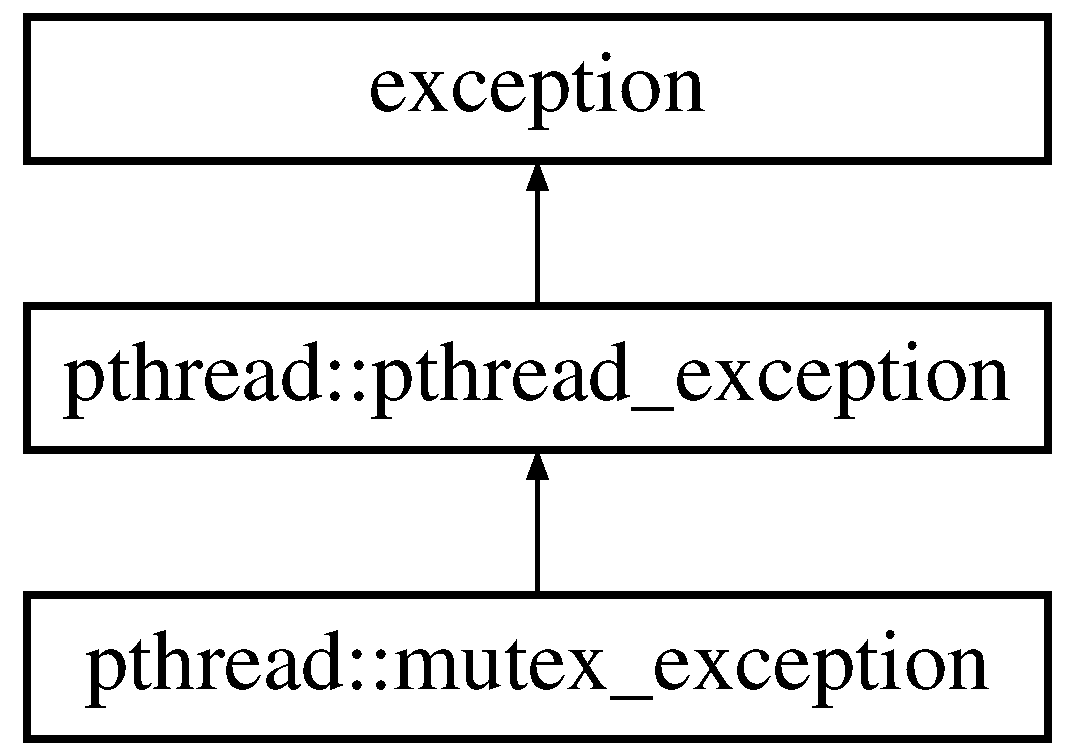
\includegraphics[height=3.000000cm]{classpthread_1_1mutex__exception}
\end{center}
\end{figure}
\subsection*{Public Member Functions}
\begin{DoxyCompactItemize}
\item 
\hyperlink{classpthread_1_1mutex__exception_a250f82ebe285c7cb28986a7086f3eae8}{mutex\+\_\+exception} (const std\+::string message, const int \hyperlink{classpthread_1_1pthread__exception_a4a869173054faca1945ac1a7729082d6}{pthread\+\_\+errno}=0)
\end{DoxyCompactItemize}


\subsection{Detailed Description}
throw to indicate that something went wrong with a mutex. 

\subsection{Constructor \& Destructor Documentation}
\hypertarget{classpthread_1_1mutex__exception_a250f82ebe285c7cb28986a7086f3eae8}{\index{pthread\+::mutex\+\_\+exception@{pthread\+::mutex\+\_\+exception}!mutex\+\_\+exception@{mutex\+\_\+exception}}
\index{mutex\+\_\+exception@{mutex\+\_\+exception}!pthread\+::mutex\+\_\+exception@{pthread\+::mutex\+\_\+exception}}
\subsubsection[{mutex\+\_\+exception}]{\setlength{\rightskip}{0pt plus 5cm}pthread\+::mutex\+\_\+exception\+::mutex\+\_\+exception (
\begin{DoxyParamCaption}
\item[{const std\+::string}]{message, }
\item[{const int}]{pthread\+\_\+errno = {\ttfamily 0}}
\end{DoxyParamCaption}
)}}\label{classpthread_1_1mutex__exception_a250f82ebe285c7cb28986a7086f3eae8}
thrown when mutex actions fail


\begin{DoxyParams}{Parameters}
{\em message} & short description \\
\hline
{\em pthread\+\_\+errno} & error returned by the pthread function \\
\hline
\end{DoxyParams}


The documentation for this class was generated from the following files\+:\begin{DoxyCompactItemize}
\item 
include/pthread/mutex.\+hpp\item 
src/mutex.\+cpp\end{DoxyCompactItemize}

\hypertarget{classpthread_1_1pthread__exception}{\section{pthread\+:\+:pthread\+\_\+exception Class Reference}
\label{classpthread_1_1pthread__exception}\index{pthread\+::pthread\+\_\+exception@{pthread\+::pthread\+\_\+exception}}
}


{\ttfamily \#include $<$exceptions.\+hpp$>$}

Inheritance diagram for pthread\+:\+:pthread\+\_\+exception\+:\begin{figure}[H]
\begin{center}
\leavevmode
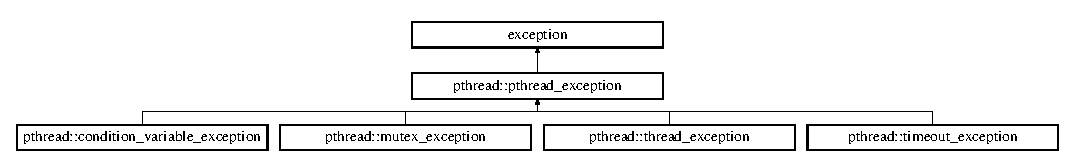
\includegraphics[height=1.794872cm]{classpthread_1_1pthread__exception}
\end{center}
\end{figure}
\subsection*{Public Member Functions}
\begin{DoxyCompactItemize}
\item 
\hyperlink{classpthread_1_1pthread__exception_ab7a3badd3201cb06efe42641a7159938}{pthread\+\_\+exception} (const string \&message, const int \hyperlink{classpthread_1_1pthread__exception_a4a869173054faca1945ac1a7729082d6}{pthread\+\_\+errno}=-\/1)
\item 
virtual const char $\ast$ \hyperlink{classpthread_1_1pthread__exception_ae54eed6aa72bac1c503554ddd857e466}{what} () const noexceptoverride
\item 
virtual int \hyperlink{classpthread_1_1pthread__exception_a4a869173054faca1945ac1a7729082d6}{pthread\+\_\+errno} ()
\item 
virtual const char $\ast$ \hyperlink{classpthread_1_1pthread__exception_afc17488e8f6160865f1beb4d6fc20d2a}{pthread\+\_\+errmsg} ()
\end{DoxyCompactItemize}


\subsection{Detailed Description}
general purpose pthread exception. 

\subsection{Constructor \& Destructor Documentation}
\hypertarget{classpthread_1_1pthread__exception_ab7a3badd3201cb06efe42641a7159938}{\index{pthread\+::pthread\+\_\+exception@{pthread\+::pthread\+\_\+exception}!pthread\+\_\+exception@{pthread\+\_\+exception}}
\index{pthread\+\_\+exception@{pthread\+\_\+exception}!pthread\+::pthread\+\_\+exception@{pthread\+::pthread\+\_\+exception}}
\subsubsection[{pthread\+\_\+exception}]{\setlength{\rightskip}{0pt plus 5cm}pthread\+::pthread\+\_\+exception\+::pthread\+\_\+exception (
\begin{DoxyParamCaption}
\item[{const string \&}]{message, }
\item[{const int}]{pthread\+\_\+errno = {\ttfamily -\/1}}
\end{DoxyParamCaption}
)}}\label{classpthread_1_1pthread__exception_ab7a3badd3201cb06efe42641a7159938}

\begin{DoxyParams}{Parameters}
{\em message} & error message \\
\hline
{\em pthread\+\_\+errno} & a pthread function return code. \\
\hline
\end{DoxyParams}


\subsection{Member Function Documentation}
\hypertarget{classpthread_1_1pthread__exception_afc17488e8f6160865f1beb4d6fc20d2a}{\index{pthread\+::pthread\+\_\+exception@{pthread\+::pthread\+\_\+exception}!pthread\+\_\+errmsg@{pthread\+\_\+errmsg}}
\index{pthread\+\_\+errmsg@{pthread\+\_\+errmsg}!pthread\+::pthread\+\_\+exception@{pthread\+::pthread\+\_\+exception}}
\subsubsection[{pthread\+\_\+errmsg}]{\setlength{\rightskip}{0pt plus 5cm}const char $\ast$ pthread\+::pthread\+\_\+exception\+::pthread\+\_\+errmsg (
\begin{DoxyParamCaption}
{}
\end{DoxyParamCaption}
)\hspace{0.3cm}{\ttfamily [virtual]}}}\label{classpthread_1_1pthread__exception_afc17488e8f6160865f1beb4d6fc20d2a}
\begin{DoxyReturn}{Returns}
related pthread\+\_\+errno error message using strerror 
\end{DoxyReturn}
\hypertarget{classpthread_1_1pthread__exception_a4a869173054faca1945ac1a7729082d6}{\index{pthread\+::pthread\+\_\+exception@{pthread\+::pthread\+\_\+exception}!pthread\+\_\+errno@{pthread\+\_\+errno}}
\index{pthread\+\_\+errno@{pthread\+\_\+errno}!pthread\+::pthread\+\_\+exception@{pthread\+::pthread\+\_\+exception}}
\subsubsection[{pthread\+\_\+errno}]{\setlength{\rightskip}{0pt plus 5cm}int pthread\+::pthread\+\_\+exception\+::pthread\+\_\+errno (
\begin{DoxyParamCaption}
{}
\end{DoxyParamCaption}
)\hspace{0.3cm}{\ttfamily [virtual]}}}\label{classpthread_1_1pthread__exception_a4a869173054faca1945ac1a7729082d6}
\begin{DoxyReturn}{Returns}
pthread error code that was at the orgin of the error 
\end{DoxyReturn}
\hypertarget{classpthread_1_1pthread__exception_ae54eed6aa72bac1c503554ddd857e466}{\index{pthread\+::pthread\+\_\+exception@{pthread\+::pthread\+\_\+exception}!what@{what}}
\index{what@{what}!pthread\+::pthread\+\_\+exception@{pthread\+::pthread\+\_\+exception}}
\subsubsection[{what}]{\setlength{\rightskip}{0pt plus 5cm}const char $\ast$ pthread\+::pthread\+\_\+exception\+::what (
\begin{DoxyParamCaption}
{}
\end{DoxyParamCaption}
) const\hspace{0.3cm}{\ttfamily [override]}, {\ttfamily [virtual]}, {\ttfamily [noexcept]}}}\label{classpthread_1_1pthread__exception_ae54eed6aa72bac1c503554ddd857e466}
\begin{DoxyReturn}{Returns}
exception's error message. 
\end{DoxyReturn}


The documentation for this class was generated from the following files\+:\begin{DoxyCompactItemize}
\item 
include/pthread/exceptions.\+hpp\item 
src/exceptions.\+cpp\end{DoxyCompactItemize}

\hypertarget{classpthread_1_1runnable}{}\section{pthread\+:\+:runnable Class Reference}
\label{classpthread_1_1runnable}\index{pthread\+::runnable@{pthread\+::runnable}}


{\ttfamily \#include $<$thread.\+hpp$>$}

\subsection*{Public Member Functions}
\begin{DoxyCompactItemize}
\item 
virtual void \hyperlink{classpthread_1_1runnable_a4e0ce933602df83c096a37974ebedf84}{run} () noexcept=0
\end{DoxyCompactItemize}


\subsection{Detailed Description}
Interface of a runnable class.

You can write code to be run through a Thread by implementing this interface. 

\subsection{Member Function Documentation}
\index{pthread\+::runnable@{pthread\+::runnable}!run@{run}}
\index{run@{run}!pthread\+::runnable@{pthread\+::runnable}}
\subsubsection[{\texorpdfstring{run() noexcept=0}{run() noexcept=0}}]{\setlength{\rightskip}{0pt plus 5cm}virtual void pthread\+::runnable\+::run (
\begin{DoxyParamCaption}
{}
\end{DoxyParamCaption}
)\hspace{0.3cm}{\ttfamily [pure virtual]}, {\ttfamily [noexcept]}}\hypertarget{classpthread_1_1runnable_a4e0ce933602df83c096a37974ebedf84}{}\label{classpthread_1_1runnable_a4e0ce933602df83c096a37974ebedf84}
This method must be overriden 

The documentation for this class was generated from the following file\+:\begin{DoxyCompactItemize}
\item 
include/pthread/thread.\+hpp\end{DoxyCompactItemize}

\hypertarget{classpthread_1_1thread}{}\section{pthread\+:\+:thread Class Reference}
\label{classpthread_1_1thread}\index{pthread\+::thread@{pthread\+::thread}}


{\ttfamily \#include $<$thread.\+hpp$>$}

\subsection*{Public Member Functions}
\begin{DoxyCompactItemize}
\item 
\hyperlink{classpthread_1_1thread_a60ac91ccf3de6e36258aa741af015095}{thread} ()
\item 
\hyperlink{classpthread_1_1thread_a978cf4c628ece8a58e75c70f85b043ea}{thread} (const \hyperlink{classpthread_1_1runnable}{runnable} \&runner)
\item 
\hyperlink{classpthread_1_1thread_a928b41a7587eba3e5e39237b4b2f655a}{thread} (\hyperlink{classpthread_1_1thread}{thread} \&\&other)
\item 
\hyperlink{classpthread_1_1thread_ab9ddf5aa6697287269dc2804051b6378}{thread} (const \hyperlink{classpthread_1_1thread}{thread} \&)=delete
\item 
virtual \hyperlink{classpthread_1_1thread_aa4920e15c3a033f94c6be462c5cbcecf}{$\sim$thread} ()
\item 
int \hyperlink{classpthread_1_1thread_a93c4105becf4dea1b00efb30cd7228af}{join} ()
\item 
bool \hyperlink{classpthread_1_1thread_a14b07d05a78157bcb5ee42fc8dd17e35}{joinable} () const 
\item 
int \hyperlink{classpthread_1_1thread_a89b64810871feee5c2d2659f3ae2f668}{cancel} ()
\item 
\hyperlink{namespacepthread_ac4b6e78f3d72c946ace7a92f3bec4101}{thread\+\_\+status} \hyperlink{classpthread_1_1thread_a3e49c7d73cb8411258790ed2fc0cd818}{status} ()
\item 
\hyperlink{classpthread_1_1thread}{thread} \& \hyperlink{classpthread_1_1thread_a09903f6b3f396f2ea046c9c1606f0f61}{operator=} (const \hyperlink{classpthread_1_1thread}{thread} \&)=delete
\item 
\hyperlink{classpthread_1_1thread}{thread} \& \hyperlink{classpthread_1_1thread_a8f9ab7d43ad9aee0368ccc4778cf40d0}{operator=} (\hyperlink{classpthread_1_1thread}{thread} \&\&other)
\end{DoxyCompactItemize}


\subsection{Detailed Description}
Handles P\+O\+S\+IX (Portable Operating System Interface) threads.

{\ttfamily  class reader\+\_\+thread\+: public runnable \{ public\+: void run() \{...\} \};}

{\ttfamily  reade\+\_\+thread rt; thread t\{rt\}; t.\+join(); } 

\subsection{Constructor \& Destructor Documentation}
\index{pthread\+::thread@{pthread\+::thread}!thread@{thread}}
\index{thread@{thread}!pthread\+::thread@{pthread\+::thread}}
\subsubsection[{\texorpdfstring{thread()}{thread()}}]{\setlength{\rightskip}{0pt plus 5cm}pthread\+::thread\+::thread (
\begin{DoxyParamCaption}
{}
\end{DoxyParamCaption}
)}\hypertarget{classpthread_1_1thread_a60ac91ccf3de6e36258aa741af015095}{}\label{classpthread_1_1thread_a60ac91ccf3de6e36258aa741af015095}
create a new thread status is no\+\_\+a\+\_\+thread \index{pthread\+::thread@{pthread\+::thread}!thread@{thread}}
\index{thread@{thread}!pthread\+::thread@{pthread\+::thread}}
\subsubsection[{\texorpdfstring{thread(const runnable \&runner)}{thread(const runnable &runner)}}]{\setlength{\rightskip}{0pt plus 5cm}pthread\+::thread\+::thread (
\begin{DoxyParamCaption}
\item[{const {\bf runnable} \&}]{runner}
\end{DoxyParamCaption}
)}\hypertarget{classpthread_1_1thread_a978cf4c628ece8a58e75c70f85b043ea}{}\label{classpthread_1_1thread_a978cf4c628ece8a58e75c70f85b043ea}
create a new thread

The new thread is made runnable, and will start executing the run routine, with.


\begin{DoxyParams}{Parameters}
{\em runner} & a class that implements the runnable interface. \\
\hline
\end{DoxyParams}
\index{pthread\+::thread@{pthread\+::thread}!thread@{thread}}
\index{thread@{thread}!pthread\+::thread@{pthread\+::thread}}
\subsubsection[{\texorpdfstring{thread(thread \&\&other)}{thread(thread &&other)}}]{\setlength{\rightskip}{0pt plus 5cm}pthread\+::thread\+::thread (
\begin{DoxyParamCaption}
\item[{{\bf thread} \&\&}]{other}
\end{DoxyParamCaption}
)}\hypertarget{classpthread_1_1thread_a928b41a7587eba3e5e39237b4b2f655a}{}\label{classpthread_1_1thread_a928b41a7587eba3e5e39237b4b2f655a}
Starts running given function in a new trhread.


\begin{DoxyParams}{Parameters}
{\em f} & function to run in thread \\
\hline
{\em args} & function paramleters/arguments. move contructor\\
\hline
\end{DoxyParams}
once moved this not a thread anymore. Status is \hyperlink{namespacepthread_ac4b6e78f3d72c946ace7a92f3bec4101a8414cd8c988083af4eabb1311df873cf}{thread\+\_\+status\+::not\+\_\+a\+\_\+thread}


\begin{DoxyParams}{Parameters}
{\em other} & thread that will be moved, on completion other is no longer a thread. \\
\hline
\end{DoxyParams}
\index{pthread\+::thread@{pthread\+::thread}!thread@{thread}}
\index{thread@{thread}!pthread\+::thread@{pthread\+::thread}}
\subsubsection[{\texorpdfstring{thread(const thread \&)=delete}{thread(const thread &)=delete}}]{\setlength{\rightskip}{0pt plus 5cm}pthread\+::thread\+::thread (
\begin{DoxyParamCaption}
\item[{const {\bf thread} \&}]{}
\end{DoxyParamCaption}
)\hspace{0.3cm}{\ttfamily [delete]}}\hypertarget{classpthread_1_1thread_ab9ddf5aa6697287269dc2804051b6378}{}\label{classpthread_1_1thread_ab9ddf5aa6697287269dc2804051b6378}
copy constructor is flagged deleted because it makes no sense to copy a thread. \index{pthread\+::thread@{pthread\+::thread}!````~thread@{$\sim$thread}}
\index{````~thread@{$\sim$thread}!pthread\+::thread@{pthread\+::thread}}
\subsubsection[{\texorpdfstring{$\sim$thread()}{~thread()}}]{\setlength{\rightskip}{0pt plus 5cm}pthread\+::thread\+::$\sim$thread (
\begin{DoxyParamCaption}
{}
\end{DoxyParamCaption}
)\hspace{0.3cm}{\ttfamily [virtual]}}\hypertarget{classpthread_1_1thread_aa4920e15c3a033f94c6be462c5cbcecf}{}\label{classpthread_1_1thread_aa4920e15c3a033f94c6be462c5cbcecf}
cleanup thread ressources. 

\subsection{Member Function Documentation}
\index{pthread\+::thread@{pthread\+::thread}!cancel@{cancel}}
\index{cancel@{cancel}!pthread\+::thread@{pthread\+::thread}}
\subsubsection[{\texorpdfstring{cancel()}{cancel()}}]{\setlength{\rightskip}{0pt plus 5cm}int pthread\+::thread\+::cancel (
\begin{DoxyParamCaption}
{}
\end{DoxyParamCaption}
)}\hypertarget{classpthread_1_1thread_a89b64810871feee5c2d2659f3ae2f668}{}\label{classpthread_1_1thread_a89b64810871feee5c2d2659f3ae2f668}
The cancel method requests the cancellation of the thread. The action depends on the cancelability of the target thread\+:

o If its cancelability is disabled, the cancellation request is set pending. o If its cancelability is deferred, the cancellation request is set pending till the thread reaches a cancellation point. o If its cancelability is asynchronous, the cancellation request is acted upon immediately; in some cases, it may result in unexpected behaviour.

The cancellation of a thread terminates it safely, using the same termination procedure as the pthread\+\_\+exit subroutine. \index{pthread\+::thread@{pthread\+::thread}!join@{join}}
\index{join@{join}!pthread\+::thread@{pthread\+::thread}}
\subsubsection[{\texorpdfstring{join()}{join()}}]{\setlength{\rightskip}{0pt plus 5cm}int pthread\+::thread\+::join (
\begin{DoxyParamCaption}
{}
\end{DoxyParamCaption}
)}\hypertarget{classpthread_1_1thread_a93c4105becf4dea1b00efb30cd7228af}{}\label{classpthread_1_1thread_a93c4105becf4dea1b00efb30cd7228af}
The join method blocks the calling thread until the thread terminates. The target thread\textquotesingle{}s termination status is returned in the status parameter.

If the target thread is already terminated, the method returns immediately.

This method does not itself cause a thread to be terminated.


\begin{DoxyExceptions}{Exceptions}
{\em \hyperlink{classpthread_1_1pthread__exception}{pthread\+\_\+exception}} & if this is not a thread or if thread\+\_\+id == this\+\_\+thread\+::get\+\_\+id(). \\
\hline
\end{DoxyExceptions}
\index{pthread\+::thread@{pthread\+::thread}!joinable@{joinable}}
\index{joinable@{joinable}!pthread\+::thread@{pthread\+::thread}}
\subsubsection[{\texorpdfstring{joinable() const }{joinable() const }}]{\setlength{\rightskip}{0pt plus 5cm}bool pthread\+::thread\+::joinable (
\begin{DoxyParamCaption}
{}
\end{DoxyParamCaption}
) const\hspace{0.3cm}{\ttfamily [inline]}}\hypertarget{classpthread_1_1thread_a14b07d05a78157bcb5ee42fc8dd17e35}{}\label{classpthread_1_1thread_a14b07d05a78157bcb5ee42fc8dd17e35}
\begin{DoxyReturn}{Returns}
true if this thread can be joined. 
\end{DoxyReturn}
\index{pthread\+::thread@{pthread\+::thread}!operator=@{operator=}}
\index{operator=@{operator=}!pthread\+::thread@{pthread\+::thread}}
\subsubsection[{\texorpdfstring{operator=(const thread \&)=delete}{operator=(const thread &)=delete}}]{\setlength{\rightskip}{0pt plus 5cm}{\bf thread}\& pthread\+::thread\+::operator= (
\begin{DoxyParamCaption}
\item[{const {\bf thread} \&}]{}
\end{DoxyParamCaption}
)\hspace{0.3cm}{\ttfamily [delete]}}\hypertarget{classpthread_1_1thread_a09903f6b3f396f2ea046c9c1606f0f61}{}\label{classpthread_1_1thread_a09903f6b3f396f2ea046c9c1606f0f61}
copy operator is flagged deleted, copying doesn\textquotesingle{}t make sense \index{pthread\+::thread@{pthread\+::thread}!operator=@{operator=}}
\index{operator=@{operator=}!pthread\+::thread@{pthread\+::thread}}
\subsubsection[{\texorpdfstring{operator=(thread \&\&other)}{operator=(thread &&other)}}]{\setlength{\rightskip}{0pt plus 5cm}{\bf thread} \& pthread\+::thread\+::operator= (
\begin{DoxyParamCaption}
\item[{{\bf thread} \&\&}]{other}
\end{DoxyParamCaption}
)}\hypertarget{classpthread_1_1thread_a8f9ab7d43ad9aee0368ccc4778cf40d0}{}\label{classpthread_1_1thread_a8f9ab7d43ad9aee0368ccc4778cf40d0}
move a thread to another thread.


\begin{DoxyParams}{Parameters}
{\em other} & thread to move, on completion it is not a thread anymore (\hyperlink{namespacepthread_ac4b6e78f3d72c946ace7a92f3bec4101a8414cd8c988083af4eabb1311df873cf}{thread\+\_\+status\+::not\+\_\+a\+\_\+thread}). \\
\hline
\end{DoxyParams}
\begin{DoxyReturn}{Returns}
thread 
\end{DoxyReturn}
\index{pthread\+::thread@{pthread\+::thread}!status@{status}}
\index{status@{status}!pthread\+::thread@{pthread\+::thread}}
\subsubsection[{\texorpdfstring{status()}{status()}}]{\setlength{\rightskip}{0pt plus 5cm}{\bf thread\+\_\+status} pthread\+::thread\+::status (
\begin{DoxyParamCaption}
{}
\end{DoxyParamCaption}
)\hspace{0.3cm}{\ttfamily [inline]}}\hypertarget{classpthread_1_1thread_a3e49c7d73cb8411258790ed2fc0cd818}{}\label{classpthread_1_1thread_a3e49c7d73cb8411258790ed2fc0cd818}
\begin{DoxyReturn}{Returns}
the status of the thread (\hyperlink{classpthread_1_1thread_a3e49c7d73cb8411258790ed2fc0cd818}{thread\+::status}). 
\end{DoxyReturn}


The documentation for this class was generated from the following files\+:\begin{DoxyCompactItemize}
\item 
include/pthread/thread.\+hpp\item 
src/thread.\+cpp\end{DoxyCompactItemize}

\hypertarget{classpthread_1_1thread__exception}{}\section{pthread\+:\+:thread\+\_\+exception Class Reference}
\label{classpthread_1_1thread__exception}\index{pthread\+::thread\+\_\+exception@{pthread\+::thread\+\_\+exception}}


{\ttfamily \#include $<$exceptions.\+hpp$>$}

Inheritance diagram for pthread\+:\+:thread\+\_\+exception\+:\begin{figure}[H]
\begin{center}
\leavevmode
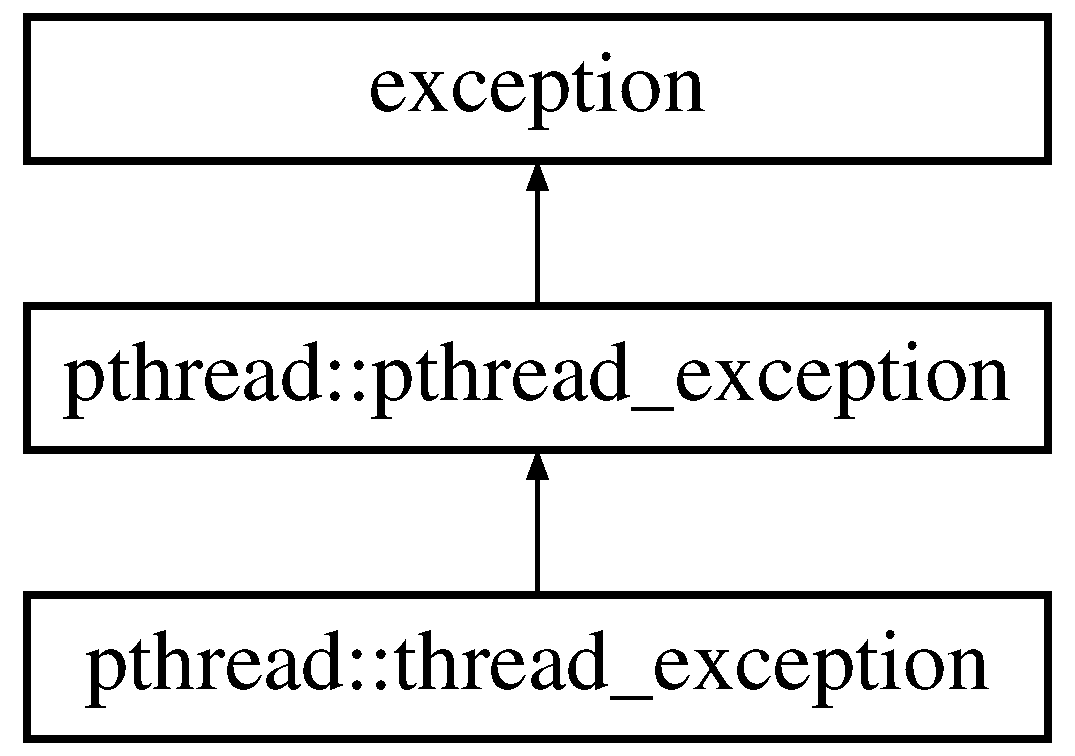
\includegraphics[height=3.000000cm]{classpthread_1_1thread__exception}
\end{center}
\end{figure}
\subsection*{Public Member Functions}
\begin{DoxyCompactItemize}
\item 
\hyperlink{classpthread_1_1thread__exception_acdaadcbdcd315d86a4466d1be460a7b7}{thread\+\_\+exception} (const std\+::string \&message, const int pthread\+\_\+error=-\/1)
\end{DoxyCompactItemize}


\subsection{Detailed Description}
thrown to indicate that something went wrong with a thread 

Definition at line 108 of file exceptions.\+hpp.



\subsection{Constructor \& Destructor Documentation}
\index{pthread\+::thread\+\_\+exception@{pthread\+::thread\+\_\+exception}!thread\+\_\+exception@{thread\+\_\+exception}}
\index{thread\+\_\+exception@{thread\+\_\+exception}!pthread\+::thread\+\_\+exception@{pthread\+::thread\+\_\+exception}}
\subsubsection[{\texorpdfstring{thread\+\_\+exception(const std\+::string \&message, const int pthread\+\_\+error=-\/1)}{thread\_exception(const std::string \&message, const int pthread\_error=-1)}}]{\setlength{\rightskip}{0pt plus 5cm}pthread\+::thread\+\_\+exception\+::thread\+\_\+exception (
\begin{DoxyParamCaption}
\item[{const std\+::string \&}]{message, }
\item[{const int}]{pthread\+\_\+error = {\ttfamily -\/1}}
\end{DoxyParamCaption}
)}\hypertarget{classpthread_1_1thread__exception_acdaadcbdcd315d86a4466d1be460a7b7}{}\label{classpthread_1_1thread__exception_acdaadcbdcd315d86a4466d1be460a7b7}

\begin{DoxyParams}{Parameters}
{\em message} & short error description. \\
\hline
{\em pthread\+\_\+error} & value return by a function in the pthread library. \\
\hline
\end{DoxyParams}


Definition at line 57 of file exceptions.\+cpp.



The documentation for this class was generated from the following files\+:\begin{DoxyCompactItemize}
\item 
include/pthread/exceptions.\+hpp\item 
src/exceptions.\+cpp\end{DoxyCompactItemize}

\hypertarget{classpthread_1_1thread__group}{}\section{pthread\+:\+:thread\+\_\+group Class Reference}
\label{classpthread_1_1thread__group}\index{pthread\+::thread\+\_\+group@{pthread\+::thread\+\_\+group}}


{\ttfamily \#include $<$thread.\+hpp$>$}

\subsection*{Public Member Functions}
\begin{DoxyCompactItemize}
\item 
\hyperlink{classpthread_1_1thread__group_ab4a8be5396449131ce2817db0e6ea2c2}{thread\+\_\+group} (bool \hyperlink{classpthread_1_1thread__group_a67df7bb484fb8657228a909a126489d3}{destructor\+\_\+joins\+\_\+first}=false) \+\_\+\+\_\+\+N\+O\+E\+X\+C\+E\+P\+T\+\_\+\+\_\+
\item 
virtual \hyperlink{classpthread_1_1thread__group_a2aeeb86d1523e2a7c175df3162331e4f}{$\sim$thread\+\_\+group} ()
\item 
void \hyperlink{classpthread_1_1thread__group_ae9fa9ce6e7b4c2222d04a446b3c23ca0}{add} (\hyperlink{classpthread_1_1abstract__thread}{abstract\+\_\+thread} $\ast$thread)
\item 
void \hyperlink{classpthread_1_1thread__group_aaba00cf80d72cd986526384482457968}{start} ()
\item 
void \hyperlink{classpthread_1_1thread__group_a39937a77e1059e352c9b39407a866f6e}{join} ()
\item 
const bool \hyperlink{classpthread_1_1thread__group_a67df7bb484fb8657228a909a126489d3}{destructor\+\_\+joins\+\_\+first} ()
\end{DoxyCompactItemize}


\subsection{Detailed Description}
Group of abstract\+\_\+threads pointers.

This helper class is in charge of handling group of threads as a whole. Method in this class apply to all threads in the group.

{\bfseries A \hyperlink{classpthread_1_1thread__group}{thread\+\_\+group} deletes the thread that were registered/added to it.}


\begin{DoxyPre}{\ttfamily 
int main(int argc, const char * argv[]) \{}\end{DoxyPre}



\begin{DoxyPre}{\ttfamily   \hyperlink{classpthread_1_1thread__group}{pthread::thread\_group} threads; // this instance will free any registered thread when it will get out of scope}\end{DoxyPre}



\begin{DoxyPre}{\ttfamily   for (auto x = 10 ; x > 0 ; x--)\{
    threads.add( new worker("herbert")); // register threads, they will run when \hyperlink{classpthread_1_1thread__group_aaba00cf80d72cd986526384482457968}{start()} is called
  \}}\end{DoxyPre}



\begin{DoxyPre}{\ttfamily   threads.start(); // start running all threads
  threads.join(); // wait for registered threads to join
\} // scope end}\end{DoxyPre}



\begin{DoxyPre}{\ttfamily   }\end{DoxyPre}
 

\subsection{Constructor \& Destructor Documentation}
\index{pthread\+::thread\+\_\+group@{pthread\+::thread\+\_\+group}!thread\+\_\+group@{thread\+\_\+group}}
\index{thread\+\_\+group@{thread\+\_\+group}!pthread\+::thread\+\_\+group@{pthread\+::thread\+\_\+group}}
\subsubsection[{\texorpdfstring{thread\+\_\+group(bool destructor\+\_\+joins\+\_\+first=false) \+\_\+\+\_\+\+N\+O\+E\+X\+C\+E\+P\+T\+\_\+\+\_\+}{thread_group(bool destructor_joins_first=false) __NOEXCEPT__}}]{\setlength{\rightskip}{0pt plus 5cm}pthread\+::thread\+\_\+group\+::thread\+\_\+group (
\begin{DoxyParamCaption}
\item[{bool}]{destructor\+\_\+joins\+\_\+first = {\ttfamily false}}
\end{DoxyParamCaption}
)}\hypertarget{classpthread_1_1thread__group_ab4a8be5396449131ce2817db0e6ea2c2}{}\label{classpthread_1_1thread__group_ab4a8be5396449131ce2817db0e6ea2c2}
Setup a thread container/list.


\begin{DoxyParams}{Parameters}
{\em destructor\+\_\+joins\+\_\+first} & if true then destructor tries to wait for all registered threads to join the calling one before deleting thread instances. \\
\hline
\end{DoxyParams}
\index{pthread\+::thread\+\_\+group@{pthread\+::thread\+\_\+group}!````~thread\+\_\+group@{$\sim$thread\+\_\+group}}
\index{````~thread\+\_\+group@{$\sim$thread\+\_\+group}!pthread\+::thread\+\_\+group@{pthread\+::thread\+\_\+group}}
\subsubsection[{\texorpdfstring{$\sim$thread\+\_\+group()}{~thread_group()}}]{\setlength{\rightskip}{0pt plus 5cm}pthread\+::thread\+\_\+group\+::$\sim$thread\+\_\+group (
\begin{DoxyParamCaption}
{}
\end{DoxyParamCaption}
)\hspace{0.3cm}{\ttfamily [virtual]}}\hypertarget{classpthread_1_1thread__group_a2aeeb86d1523e2a7c175df3162331e4f}{}\label{classpthread_1_1thread__group_a2aeeb86d1523e2a7c175df3162331e4f}
delete all \hyperlink{classpthread_1_1abstract__thread}{abstract\+\_\+thread} referenced by the \hyperlink{classpthread_1_1thread__group}{thread\+\_\+group}.

If destructor\+\_\+joins\+\_\+first is true then the method \hyperlink{classpthread_1_1abstract__thread_aedac81bb9eb76ba92c49c48d797ea25b}{abstract\+\_\+thread\+::join()} is called before deleting the referenced \hyperlink{classpthread_1_1abstract__thread}{abstract\+\_\+thread}. 

\subsection{Member Function Documentation}
\index{pthread\+::thread\+\_\+group@{pthread\+::thread\+\_\+group}!add@{add}}
\index{add@{add}!pthread\+::thread\+\_\+group@{pthread\+::thread\+\_\+group}}
\subsubsection[{\texorpdfstring{add(abstract\+\_\+thread $\ast$thread)}{add(abstract_thread *thread)}}]{\setlength{\rightskip}{0pt plus 5cm}void pthread\+::thread\+\_\+group\+::add (
\begin{DoxyParamCaption}
\item[{{\bf pthread\+::abstract\+\_\+thread} $\ast$}]{thread}
\end{DoxyParamCaption}
)}\hypertarget{classpthread_1_1thread__group_ae9fa9ce6e7b4c2222d04a446b3c23ca0}{}\label{classpthread_1_1thread__group_ae9fa9ce6e7b4c2222d04a446b3c23ca0}

\begin{DoxyParams}{Parameters}
{\em thread} & add/register a thread to the group. \\
\hline
\end{DoxyParams}
\index{pthread\+::thread\+\_\+group@{pthread\+::thread\+\_\+group}!destructor\+\_\+joins\+\_\+first@{destructor\+\_\+joins\+\_\+first}}
\index{destructor\+\_\+joins\+\_\+first@{destructor\+\_\+joins\+\_\+first}!pthread\+::thread\+\_\+group@{pthread\+::thread\+\_\+group}}
\subsubsection[{\texorpdfstring{destructor\+\_\+joins\+\_\+first()}{destructor_joins_first()}}]{\setlength{\rightskip}{0pt plus 5cm}const bool pthread\+::thread\+\_\+group\+::destructor\+\_\+joins\+\_\+first (
\begin{DoxyParamCaption}
{}
\end{DoxyParamCaption}
)\hspace{0.3cm}{\ttfamily [inline]}}\hypertarget{classpthread_1_1thread__group_a67df7bb484fb8657228a909a126489d3}{}\label{classpthread_1_1thread__group_a67df7bb484fb8657228a909a126489d3}
return if \hyperlink{classpthread_1_1thread__group}{thread\+\_\+group} should wait for all referenced \hyperlink{classpthread_1_1abstract__thread}{abstract\+\_\+thread} terminate \index{pthread\+::thread\+\_\+group@{pthread\+::thread\+\_\+group}!join@{join}}
\index{join@{join}!pthread\+::thread\+\_\+group@{pthread\+::thread\+\_\+group}}
\subsubsection[{\texorpdfstring{join()}{join()}}]{\setlength{\rightskip}{0pt plus 5cm}void pthread\+::thread\+\_\+group\+::join (
\begin{DoxyParamCaption}
{}
\end{DoxyParamCaption}
)}\hypertarget{classpthread_1_1thread__group_a39937a77e1059e352c9b39407a866f6e}{}\label{classpthread_1_1thread__group_a39937a77e1059e352c9b39407a866f6e}
what for all threads to join the caller of this method. \index{pthread\+::thread\+\_\+group@{pthread\+::thread\+\_\+group}!start@{start}}
\index{start@{start}!pthread\+::thread\+\_\+group@{pthread\+::thread\+\_\+group}}
\subsubsection[{\texorpdfstring{start()}{start()}}]{\setlength{\rightskip}{0pt plus 5cm}void pthread\+::thread\+\_\+group\+::start (
\begin{DoxyParamCaption}
{}
\end{DoxyParamCaption}
)}\hypertarget{classpthread_1_1thread__group_aaba00cf80d72cd986526384482457968}{}\label{classpthread_1_1thread__group_aaba00cf80d72cd986526384482457968}
start run all registered threads. \begin{DoxySeeAlso}{See also}
\hyperlink{classpthread_1_1thread__group_ae9fa9ce6e7b4c2222d04a446b3c23ca0}{add(abstract\+\_\+thread $\ast$thread)} 
\end{DoxySeeAlso}


The documentation for this class was generated from the following files\+:\begin{DoxyCompactItemize}
\item 
include/pthread/thread.\+hpp\item 
src/thread.\+cpp\end{DoxyCompactItemize}

\hypertarget{classpthread_1_1timeout__exception}{\section{pthread\+:\+:timeout\+\_\+exception Class Reference}
\label{classpthread_1_1timeout__exception}\index{pthread\+::timeout\+\_\+exception@{pthread\+::timeout\+\_\+exception}}
}


{\ttfamily \#include $<$exceptions.\+hpp$>$}

Inheritance diagram for pthread\+:\+:timeout\+\_\+exception\+:\begin{figure}[H]
\begin{center}
\leavevmode
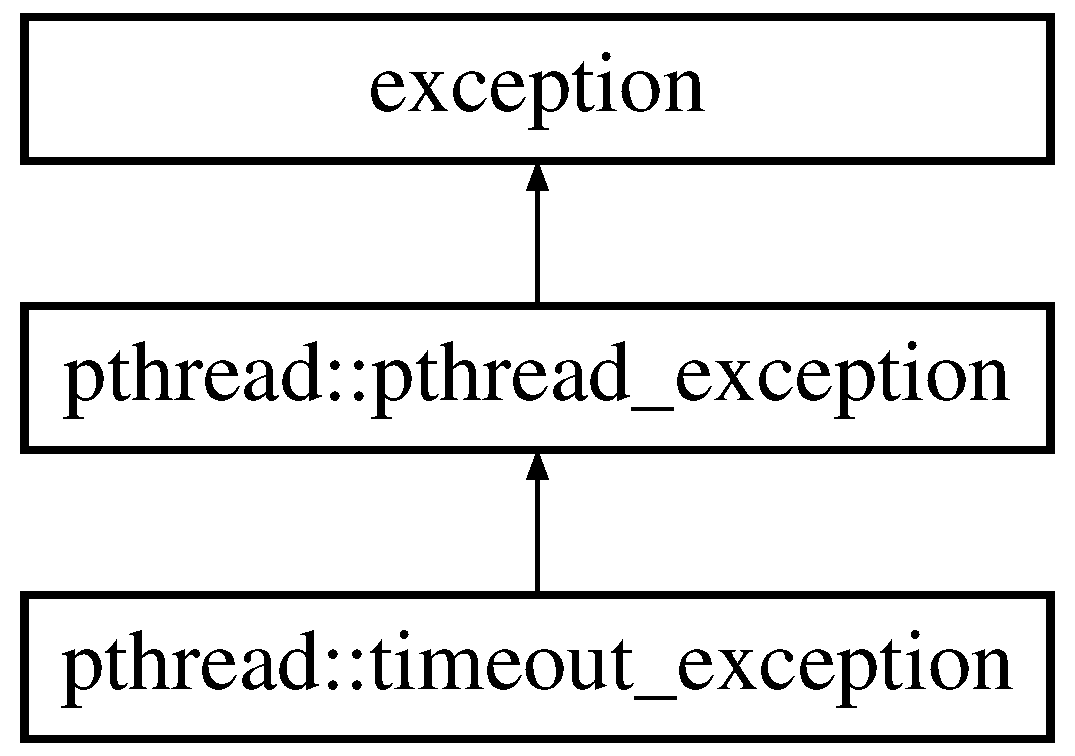
\includegraphics[height=3.000000cm]{classpthread_1_1timeout__exception}
\end{center}
\end{figure}
\subsection*{Public Member Functions}
\begin{DoxyCompactItemize}
\item 
\hyperlink{classpthread_1_1timeout__exception_a21ab48587bb22b4a0f7132dfc1f17a3d}{timeout\+\_\+exception} (const string \&message)
\end{DoxyCompactItemize}


\subsection{Detailed Description}
pthread operation timed out. 

\subsection{Constructor \& Destructor Documentation}
\hypertarget{classpthread_1_1timeout__exception_a21ab48587bb22b4a0f7132dfc1f17a3d}{\index{pthread\+::timeout\+\_\+exception@{pthread\+::timeout\+\_\+exception}!timeout\+\_\+exception@{timeout\+\_\+exception}}
\index{timeout\+\_\+exception@{timeout\+\_\+exception}!pthread\+::timeout\+\_\+exception@{pthread\+::timeout\+\_\+exception}}
\subsubsection[{timeout\+\_\+exception}]{\setlength{\rightskip}{0pt plus 5cm}pthread\+::timeout\+\_\+exception\+::timeout\+\_\+exception (
\begin{DoxyParamCaption}
\item[{const string \&}]{message}
\end{DoxyParamCaption}
)}}\label{classpthread_1_1timeout__exception_a21ab48587bb22b4a0f7132dfc1f17a3d}
thrown when a time out occurs.


\begin{DoxyParams}{Parameters}
{\em message} & timeout condition \\
\hline
\end{DoxyParams}


The documentation for this class was generated from the following files\+:\begin{DoxyCompactItemize}
\item 
include/pthread/exceptions.\+hpp\item 
src/exceptions.\+cpp\end{DoxyCompactItemize}

%--- End generated contents ---

% Index
\backmatter
\newpage
\phantomsection
\clearemptydoublepage
\addcontentsline{toc}{chapter}{Index}
\printindex

\end{document}
